\documentclass[11pt,a4paper]{article}

% Image mode: pdf.
% Image paths stay relative. In PDF mode, place same-basename PDF conversions
% of the chapter SVG files in the assets/ directory beside this source.

\usepackage{iftex}
\ifPDFTeX
  \PackageError{handout}{This template requires XeTeX or Tectonic}{Compile with xelatex or tectonic.}
\fi

\usepackage[a4paper,top=18mm,bottom=20mm,left=20mm,right=20mm,headsep=6mm]{geometry}
\usepackage{fontspec}
\usepackage{xeCJK}
\usepackage{amsmath}
\usepackage{unicode-math}

% Font settings are intentionally visible in the generated .tex file.
% These defaults target the macOS machine used for the released PDF.
% Change the family names when compiling on another system.
\setmainfont{Songti TC}
\setsansfont{Heiti TC}
\setmonofont{Menlo}
\setCJKmainfont{Songti TC}
\setCJKsansfont{Heiti TC}
\setCJKmonofont{Heiti TC}
\setmathfont{STIX Two Math}
\XeTeXlinebreaklocale "zh"
\XeTeXlinebreakskip=0pt plus 1pt

\usepackage{xcolor}
\definecolor{HandoutBlue}{HTML}{215A91}
\definecolor{HandoutBlueLight}{HTML}{EEF5FC}
\definecolor{HandoutGreen}{HTML}{39715A}
\definecolor{HandoutGreenLight}{HTML}{EFF8F3}
\definecolor{HandoutGold}{HTML}{8A641C}
\definecolor{HandoutGoldLight}{HTML}{FFF8E8}
\definecolor{HandoutInk}{HTML}{253142}
\definecolor{HandoutMuted}{HTML}{667085}

\usepackage{graphicx}
\makeatletter
% Pandoc 3 emits an accessibility `alt` key for raster/PDF images. Older
% graphicx releases do not know that key, so accept it without changing layout.
\@ifundefined{KV@Gin@alt}{\define@key{Gin}{alt}{}}{}
\newsavebox\pandoc@box
\newcommand*\pandocbounded[1]{%
  \sbox\pandoc@box{#1}%
  \Gscale@div\@tempa{\textheight}{\dimexpr\ht\pandoc@box+\dp\pandoc@box\relax}%
  \Gscale@div\@tempb{\linewidth}{\wd\pandoc@box}%
  \ifdim\@tempb\p@<\@tempa\p@\let\@tempa\@tempb\fi
  \ifdim\@tempa\p@<\p@\scalebox{\@tempa}{\usebox\pandoc@box}%
  \else\usebox{\pandoc@box}%
  \fi
}
\makeatother
\usepackage{float}
\floatplacement{figure}{H}
% Pandoc uses LTcaptype=none for uncaptioned longtables. The caption package
% expects that name to exist as a counter even though it is never displayed.
\newcounter{none}
\usepackage{caption}
\captionsetup[figure]{labelformat=empty,labelsep=none,font=small}

\usepackage{booktabs,longtable,array,calc}
\usepackage{etoolbox}
\makeatletter
\patchcmd\longtable{\par}{\if@noskipsec\mbox{}\fi\par}{}{}
\makeatother

\usepackage[most]{tcolorbox}
\tcbuselibrary{breakable,skins}
\newtcolorbox{HandoutLearningMap}{
  enhanced,breakable,colback=HandoutBlueLight,colframe=HandoutBlue,
  boxrule=0.8pt,arc=1.5mm,left=3mm,right=3mm,top=2mm,bottom=2mm,
  before skip=8pt,after skip=10pt
}
\newtcolorbox{HandoutWorkedExample}{
  enhanced,breakable,colback=HandoutGreenLight,colframe=HandoutGreen,
  boxrule=0.65pt,arc=1.5mm,left=3mm,right=3mm,top=2mm,bottom=2mm,
  before skip=8pt,after skip=10pt
}
\newtcolorbox{HandoutSelfCheck}{
  enhanced,breakable,colback=HandoutGoldLight,colframe=HandoutGold,
  boxrule=0.65pt,arc=1.5mm,left=3mm,right=3mm,top=2mm,bottom=2mm,
  before skip=8pt,after skip=10pt
}

\usepackage{titlesec}
\titleformat{\section}{\sffamily\bfseries\Large\color{HandoutBlue}}{}{0pt}{}
\titleformat{\subsection}{\sffamily\bfseries\large\color{HandoutInk}}{}{0pt}{}
\titleformat{\subsubsection}{\sffamily\bfseries\normalsize\color{HandoutInk}}{}{0pt}{}
\titlespacing*{\section}{0pt}{1.4em}{0.55em}
\titlespacing*{\subsection}{0pt}{1.15em}{0.45em}
\titlespacing*{\subsubsection}{0pt}{0.9em}{0.35em}
\setcounter{secnumdepth}{-\maxdimen}

\usepackage{hyperref}
\usepackage{bookmark}
\IfFileExists{xurl.sty}{\usepackage{xurl}}{}
\urlstyle{same}
\hypersetup{
  colorlinks=true,
  linkcolor=HandoutBlue,
  urlcolor=HandoutBlue,
  citecolor=HandoutBlue,
  pdftitle={數A4-4 矩陣},
  pdfsubject={數學},
  pdfcreator={Pandoc with the HighSchooContent LaTeX template}
}

\setlength{\parindent}{0pt}
\setlength{\parskip}{0.55em plus 0.15em minus 0.1em}
\setlength{\emergencystretch}{3em}
\setlength{\LTpre}{0.5em}
\setlength{\LTpost}{0.5em}
\renewcommand{\arraystretch}{1.18}
\providecommand{\tightlist}{%
  \setlength{\itemsep}{0pt}\setlength{\parskip}{0pt}}
\pagestyle{plain}


\begin{document}

\begin{tcolorbox}[
  enhanced,colback=white,colframe=HandoutBlue,boxrule=1.1pt,arc=2mm,
  borderline west={3pt}{0pt}{HandoutBlue},left=5mm,right=4mm,top=4mm,bottom=4mm
]
{\sffamily\small\bfseries\color{HandoutBlue}學生講義}\par
{\sffamily\bfseries\LARGE\color{HandoutInk}數A4-4 矩陣}\par
\vspace{0.35em}{\large 用列運算解多變數系統，以矩陣組合資料、機率狀態與平面變換}\par
\vspace{0.45em}{\small\color{HandoutMuted}%
科目：數學
\quad 課程：普通高中數學A 第四冊
\quad 版本：學生版｜核心＋理解
\quad 校訂：2026-08-29
}\par
\vspace{0.25em}{\small\color{HandoutMuted}範圍：現行數學 A 第四冊第四章；涵蓋高斯消去法、矩陣運算、二階反方陣、轉移矩陣與二階線性變換}\par
\end{tcolorbox}


矩陣把一批有固定索引的數字放進同一個運算物件。聯立方程式的係數、不同商品的數量與單價、人口在區域間的流動比例，以及平面圖形的伸縮與旋轉，看似屬於不同問題，實際上都能寫成矩陣與向量的乘法。

矩陣的價值在於保留結構：列、行的位置說明每個數字代表什麼；乘法把共享索引逐項相乘後加總；反方陣描述可逆的資訊變換；矩陣冪則把同一規則重複作用多次。

\begin{HandoutLearningMap}

\subsection{本章問題與能力}\label{ux672cux7ae0ux554fux984cux8207ux80fdux529b}

\begin{enumerate}
\def\labelenumi{\arabic{enumi}.}
\tightlist
\item
  高斯消去法為何保持方程組的解？消去後如何判斷唯一解、無限多組解與無解？
\item
  矩陣的階數與索引如何保存資料意義？加法、係數積與乘法各自對應什麼操作？
\item
  何時二階方陣具有反方陣？行列式為何同時控制可逆性與面積倍率？
\item
  轉移矩陣如何把本期狀態推到下一期，並分析多期後的比例？
\item
  二階矩陣如何決定平面線性變換？伸縮、鏡射、旋轉、推移與合成的矩陣從何而來？
\end{enumerate}

\end{HandoutLearningMap}

\section{1. 高斯消去法、解型與線性組合}\label{ux9ad8ux65afux6d88ux53bbux6cd5ux89e3ux578bux8207ux7ddaux6027ux7d44ux5408}

\subsection{1.1 方程式操作與增廣矩陣}\label{ux65b9ux7a0bux5f0fux64cdux4f5cux8207ux589eux5ee3ux77e9ux9663}

三元一次方程組可寫成

\[
\begin{cases}
a_{11}x+a_{12}y+a_{13}z=b_1,\\
a_{21}x+a_{22}y+a_{23}z=b_2,\\
a_{31}x+a_{32}y+a_{33}z=b_3.
\end{cases}
\]

固定未知數順序 \(x,y,z\) 後，只記錄係數與常數項，得到增廣矩陣

\[
\left[
\begin{array}{ccc|c}
a_{11}&a_{12}&a_{13}&b_1\\
a_{21}&a_{22}&a_{23}&b_2\\
a_{31}&a_{32}&a_{33}&b_3
\end{array}
\right].
\]

高斯消去法使用三種基本列運算：

\begin{enumerate}
\def\labelenumi{\arabic{enumi}.}
\tightlist
\item
  交換兩列：\(R_i\leftrightarrow R_j\)；
\item
  一列乘非零常數：\(R_i\leftarrow cR_i\)，其中 \(c\ne0\)；
\item
  一列加上另一列的倍數：\(R_i\leftarrow R_i+cR_j\)。
\end{enumerate}

每種操作都有逆操作，因此操作前後的方程組具有相同解集合。消去的目標是讓樞紐位置逐列向右移，形成階梯形；再由最下方含樞紐的方程式往上代回。

\begin{figure}
\centering
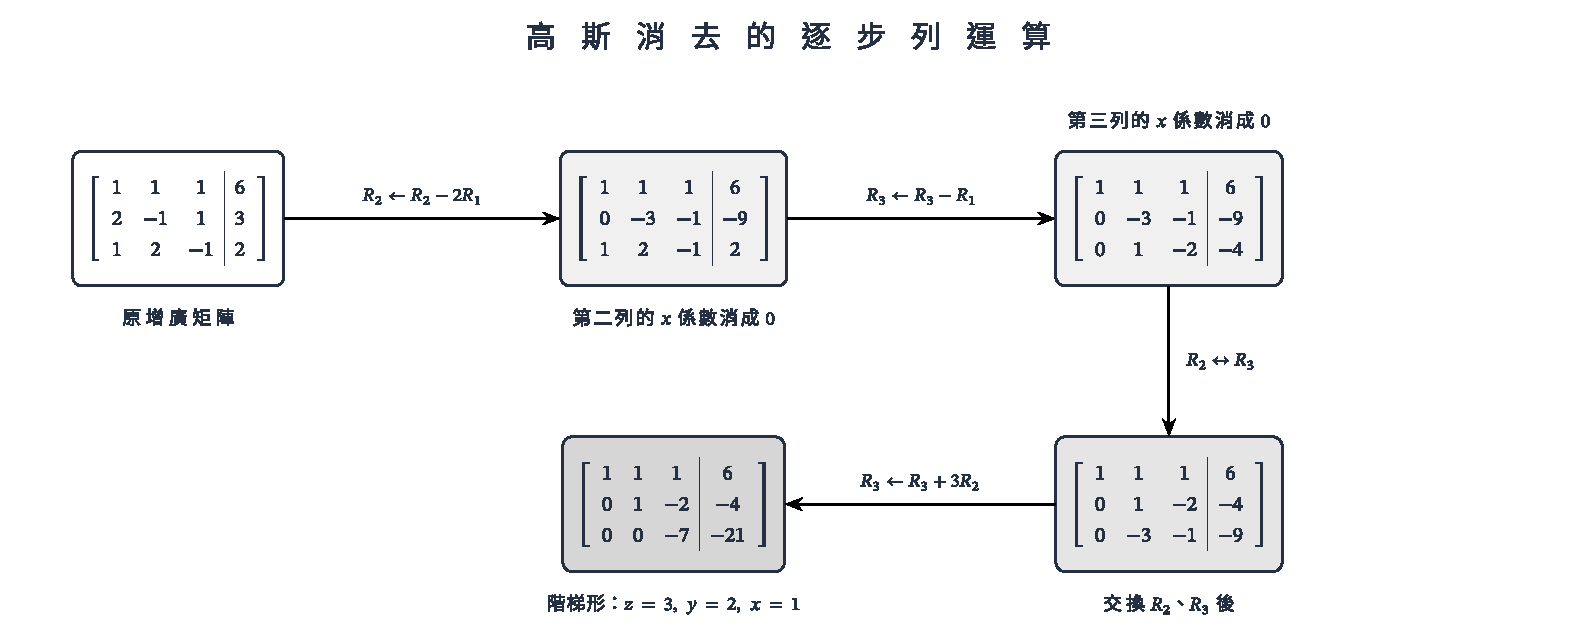
\includegraphics[width=0.96\linewidth,height=\textheight,keepaspectratio,alt={圖 1｜每一步列運算都有逆操作；圖中的方程組由階梯形讀得 z=3,y=2,x=1。}]{assets/數A4-4-高斯消去流程.pdf}
\caption{圖 1｜每一步列運算都有逆操作；圖中的方程組由階梯形讀得 \(z=3,y=2,x=1\)。}
\end{figure}

\begin{HandoutWorkedExample}

\subsection{完整示範｜列運算為何保存解集合}\label{ux5b8cux6574ux793aux7bc4ux5217ux904bux7b97ux70baux4f55ux4fddux5b58ux89e3ux96c6ux5408}

方程式 \(E_1=0\)、\(E_2=0\) 的共同解，同時滿足

\[
E_2-3E_1=0.
\]

因此把第二式改成 \(E_2-3E_1=0\) 後，每個原解仍是新方程組的解。反過來，若某組數滿足

\[
E_1=0,\qquad E_2-3E_1=0,
\]

則把第二個等式加回 \(3E_1=0\)，可得 \(E_2=0\)。兩個解集合完全相同。

交換兩式的逆操作仍是交換；乘 \(c\ne0\) 的逆操作是乘 \(1/c\)。三種列運算都可逆，這就是高斯消去過程能持續改寫方程組的依據。

\end{HandoutWorkedExample}

\begin{HandoutWorkedExample}

\subsection{完整示範｜三元一次方程組的唯一解}\label{ux5b8cux6574ux793aux7bc4ux4e09ux5143ux4e00ux6b21ux65b9ux7a0bux7d44ux7684ux552fux4e00ux89e3}

解方程組

\[
\begin{cases}
x+y+z=6,\\
2x-y+z=3,\\
x+2y-z=2.
\end{cases}
\]

增廣矩陣為

\[
\left[
\begin{array}{ccc|c}
1&1&1&6\\
2&-1&1&3\\
1&2&-1&2
\end{array}
\right].
\]

先消去第二列的 \(x\)：

\[
R_2\leftarrow R_2-2R_1,
\]

\[
\left[
\begin{array}{ccc|c}
1&1&1&6\\
0&-3&-1&-9\\
1&2&-1&2
\end{array}
\right].
\]

\clearpage

再消去第三列的 \(x\)：

\[
R_3\leftarrow R_3-R_1,
\]

\[
\left[
\begin{array}{ccc|c}
1&1&1&6\\
0&-3&-1&-9\\
0&1&-2&-4
\end{array}
\right].
\]

交換第二、三列：

\[
R_2\leftrightarrow R_3,
\]

\[
\left[
\begin{array}{ccc|c}
1&1&1&6\\
0&1&-2&-4\\
0&-3&-1&-9
\end{array}
\right].
\]

最後消去第三列的 \(y\)：

\[
R_3\leftarrow R_3+3R_2,
\]

\[
\left[
\begin{array}{ccc|c}
1&1&1&6\\
0&1&-2&-4\\
0&0&-7&-21
\end{array}
\right].
\]

由第三列得 \(z=3\)；代入第二列得 \(y-6=-4\)，所以 \(y=2\)；再代入第一列得 \(x=1\)。因此

\[
\boxed{(x,y,z)=(1,2,3)}.
\]

代回三個原式分別得到 \(6,3,2\)，與右側常數一致。

\end{HandoutWorkedExample}

\subsection{1.2 消去後的三種解型}\label{ux6d88ux53bbux5f8cux7684ux4e09ux7a2eux89e3ux578b}

消去後需讀取兩類資訊：

\begin{itemize}
\tightlist
\item
  每個未知數所在行是否出現樞紐；
\item
  是否出現形如 \(\left[\begin{array}{ccc|c}0&0&0&c\end{array}\right]\) 且 \(c\ne0\) 的矛盾列。
\end{itemize}

若每個未知數都有樞紐，得到唯一解。若沒有矛盾列且存在缺少樞紐的未知數，該未知數可設為參數，得到無限多組解。若出現 \(0=c\)、\(c\ne0\)，方程組無解。

\begin{figure}
\centering
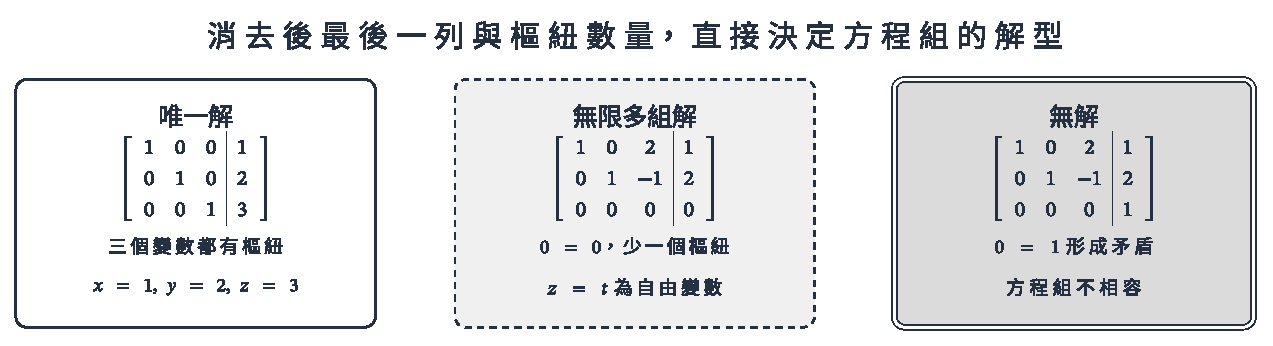
\includegraphics[width=0.96\linewidth,height=\textheight,keepaspectratio,alt={圖 2｜三種階梯形的最後一列分別給出樞紐、自由變數與矛盾式。}]{assets/數A4-4-解型分類.pdf}
\caption{圖 2｜三種階梯形的最後一列分別給出樞紐、自由變數與矛盾式。}
\end{figure}

\begin{HandoutWorkedExample}

\subsection{完整示範｜自由變數與參數解}\label{ux5b8cux6574ux793aux7bc4ux81eaux7531ux8b8aux6578ux8207ux53c3ux6578ux89e3}

某方程組經列運算後得到

\[
\left[
\begin{array}{ccc|c}
1&0&2&1\\
0&1&-1&2\\
0&0&0&0
\end{array}
\right].
\]

對應方程式為

\[
x+2z=1,\qquad y-z=2.
\]

\(z\) 所在行沒有樞紐，令 \(z=t\)，其中 \(t\in\mathbb R\)，便得到

\[
x=1-2t,\qquad y=2+t,\qquad z=t.
\]

所以解集合為

\[
\boxed{(x,y,z)=(1-2t,\;2+t,\;t),\quad t\in\mathbb R}.
\]

不同 \(t\) 對應不同解，最後一列 \(0=0\) 只提供相容性，不增加限制。

\end{HandoutWorkedExample}

\begin{HandoutWorkedExample}

\subsection{完整示範｜含參數方程組的解型}\label{ux5b8cux6574ux793aux7bc4ux542bux53c3ux6578ux65b9ux7a0bux7d44ux7684ux89e3ux578b}

已知某方程組的增廣矩陣可化為

\[
\left[
\begin{array}{ccc|c}
1&2&0&3\\
0&1&-1&1\\
0&0&0&a-4
\end{array}
\right].
\]

當 \(a\ne4\) 時，最後一列表示 \(0=a-4\)，形成矛盾，所以無解。

當 \(a=4\) 時，最後一列成為 \(0=0\)。令 \(z=t\)，由第二列得 \(y=1+t\)；由第一列得

\[
x+2(1+t)=3
\quad\Longrightarrow\quad
x=1-2t.
\]

因此

\[
\boxed{
\begin{cases}
\text{無解}, & a\ne4,\\
(x,y,z)=(1-2t,\ 1+t,\ t),\quad t\in\mathbb R, & a=4
\end{cases}
}.
\]

\end{HandoutWorkedExample}

\subsection{1.3 插值：由資料點求模型係數}\label{ux63d2ux503cux7531ux8cc7ux6599ux9edeux6c42ux6a21ux578bux4fc2ux6578}

給定三個橫坐標互異的點，可設次數不超過二次的多項式

\[
f(x)=ax^2+bx+c,
\]

再把三點依序代入，形成關於 \(a,b,c\) 的三元一次方程組。這種「模型對參數是線性的」結構廣泛用於校正曲線、資料插值與參數估計。

\begin{figure}
\centering
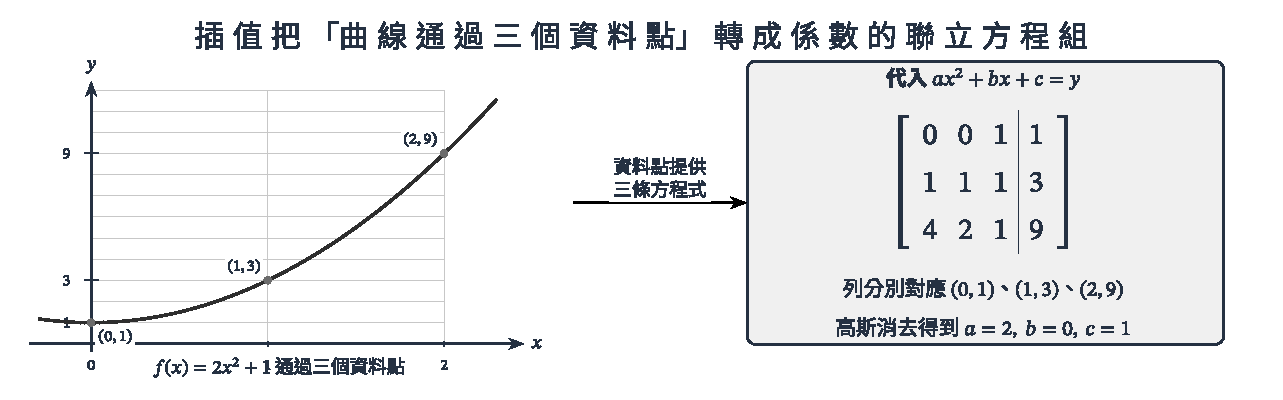
\includegraphics[width=0.92\linewidth,height=\textheight,keepaspectratio,alt={圖 3｜三個資料點代入 ax\^{}2+bx+c，高斯消去後得到通過三點的二次多項式。}]{assets/數A4-4-插值多項式.pdf}
\caption{圖 3｜三個資料點代入 \(ax^2+bx+c\)，高斯消去後得到通過三點的二次多項式。}
\end{figure}

\begin{HandoutWorkedExample}

\subsection{完整示範｜通過三點的二次多項式}\label{ux5b8cux6574ux793aux7bc4ux901aux904eux4e09ux9edeux7684ux4e8cux6b21ux591aux9805ux5f0f}

求通過 \((0,1),(1,3),(2,9)\) 的二次多項式。

令 \(f(x)=ax^2+bx+c\)。代入三點：

\[
\begin{cases}
c=1,\\
a+b+c=3,\\
4a+2b+c=9.
\end{cases}
\]

增廣矩陣為

\[
\left[
\begin{array}{ccc|c}
0&0&1&1\\
1&1&1&3\\
4&2&1&9
\end{array}
\right].
\]

由 \(c=1\)，後兩式化為 \(a+b=2\)、\(2a+b=4\)，相減得 \(a=2\)，進而 \(b=0\)。所以

\[
\boxed{f(x)=2x^2+1}.
\]

代入 \(x=0,1,2\) 分別得到 \(1,3,9\)。

\end{HandoutWorkedExample}

\begin{HandoutWorkedExample}

\subsection{完整示範｜線性校正模型}\label{ux5b8cux6574ux793aux7bc4ux7ddaux6027ux6821ux6b63ux6a21ux578b}

某感測器真值 \(x\) 與讀值 \(y\) 假設滿足 \(y=mx+b\)。兩個校正點為 \((2,5.1)\) 與 \((8,16.8)\)。求 \(m,b\)。

\[
\begin{cases}
2m+b=5.1,\\
8m+b=16.8.
\end{cases}
\]

第二式減第一式：

\[
6m=11.7
\quad\Longrightarrow\quad
m=1.95.
\]

再代回 \(2m+b=5.1\)：

\[
b=5.1-3.9=1.2.
\]

校正式為

\[
\boxed{y=1.95x+1.2}.
\]

若要由讀值反求真值，可解 \(x=(y-1.2)/1.95\)；這是可逆線性模型的最簡單例子。

\end{HandoutWorkedExample}

\subsection{1.4 空間向量的線性組合}\label{ux7a7aux9593ux5411ux91cfux7684ux7ddaux6027ux7d44ux5408}

若

\[
\vec d=x\vec a+y\vec b+z\vec c,
\]

比較三個坐標分量後就得到三元一次方程組。方程組的解型同時具有幾何意義：

\begin{itemize}
\tightlist
\item
  唯一解：\(\vec a,\vec b,\vec c\) 提供三個獨立方向，\(\vec d\) 的表示唯一；
\item
  無限多組解：三個向量的方向資訊有重複，且 \(\vec d\) 仍落在它們張成的範圍內；
\item
  無解：\(\vec d\) 位於它們張成範圍之外。
\end{itemize}

\begin{HandoutWorkedExample}

\subsection{完整示範｜求線性組合係數}\label{ux5b8cux6574ux793aux7bc4ux6c42ux7ddaux6027ux7d44ux5408ux4fc2ux6578}

給定

\[
\vec a=(1,0,1),\quad
\vec b=(0,1,1),\quad
\vec c=(1,1,0),\quad
\vec d=(5,4,3).
\]

設 \(\vec d=x\vec a+y\vec b+z\vec c\)。比較坐標：

\[
\begin{cases}
x+z=5,\\
y+z=4,\\
x+y=3.
\end{cases}
\]

前兩式相加再減第三式，得 \(2z=6\)，所以 \(z=3\)。接著 \(x=2\)、\(y=1\)。因此

\[
\boxed{\vec d=2\vec a+\vec b+3\vec c}.
\]

直接相加 \((2,0,2)+(0,1,1)+(3,3,0)=(5,4,3)\)，與 \(\vec d\) 一致。

\end{HandoutWorkedExample}

\begin{HandoutWorkedExample}

\subsection{完整示範｜共面向量造成不唯一表示}\label{ux5b8cux6574ux793aux7bc4ux5171ux9762ux5411ux91cfux9020ux6210ux4e0dux552fux4e00ux8868ux793a}

令

\[
\vec a=(1,0,0),\quad
\vec b=(0,1,0),\quad
\vec c=(1,1,0),\quad
\vec d=(3,4,0).
\]

設 \(\vec d=x\vec a+y\vec b+z\vec c\)，得到

\[
x+z=3,\qquad y+z=4,\qquad 0=0.
\]

令 \(z=t\)，則

\[
x=3-t,\qquad y=4-t.
\]

所以

\[
\boxed{\vec d=(3-t)\vec a+(4-t)\vec b+t\vec c,\quad t\in\mathbb R}.
\]

因為 \(\vec c=\vec a+\vec b\)，三個方向中有重複資訊；改變 \(t\) 只是重新分配同一組向量總和。

\end{HandoutWorkedExample}

\begin{HandoutSelfCheck}

\subsection{分節練習｜高斯消去、插值與線性組合}\label{ux5206ux7bc0ux7df4ux7fd2ux9ad8ux65afux6d88ux53bbux63d2ux503cux8207ux7ddaux6027ux7d44ux5408}

\begin{enumerate}
\def\labelenumi{\arabic{enumi}.}
\tightlist
\item
  用增廣矩陣解
  \[
  \begin{cases}
  x+y+z=4,\\
  2x-y+z=3,\\
  x+2y-z=1.
  \end{cases}
  \]
\item
  判斷下列階梯形所代表方程組的解型，若有無限多組解，寫出參數解：
  \[
  \left[
  \begin{array}{ccc|c}
  1&0&-2&3\\
  0&1&1&-1\\
  0&0&0&0
  \end{array}
  \right].
  \]
\item
  某方程組可化為最後一列 \(\left[\begin{array}{ccc|c}0&0&0&2k-6\end{array}\right]\)，其餘兩列有兩個樞紐。分別討論 \(k\) 的條件與解型。
\item
  求通過 \((0,2),(1,2),(2,6)\) 的二次多項式 \(f(x)=ax^2+bx+c\)。
\item
  已知 \(y=mx+b\) 通過 \((3,7)\) 與 \((7,19)\)，求 \(m,b\)。
\item
  令 \(\vec a=(1,1,0)\)、\(\vec b=(1,0,1)\)、\(\vec c=(0,1,1)\)、\(\vec d=(5,4,3)\)，把 \(\vec d\) 表示為 \(\vec a,\vec b,\vec c\) 的線性組合。
\end{enumerate}

\textbf{解答}

\begin{enumerate}
\def\labelenumi{\arabic{enumi}.}
\tightlist
\item
  消去後可得 \(z=2,y=1,x=1\)，所以 \(\boxed{(1,1,2)}\)。
\item
  令 \(z=t\)，則 \(x=3+2t\)、\(y=-1-t\)，所以 \(\boxed{(x,y,z)=(3+2t,-1-t,t)}\)。
\item
  \(k\ne3\) 時最後一列為矛盾式，故無解；\(k=3\) 時有兩個樞紐與一個自由變數，故有無限多組解。
\item
  \(c=2\)、\(a+b=0\)、\(4a+2b=4\)，解得 \(a=2,b=-2\)，故 \(\boxed{f(x)=2x^2-2x+2}\)。
\item
  斜率 \(m=(19-7)/(7-3)=3\)，代回得 \(b=-2\)，故 \(\boxed{y=3x-2}\)。
\item
  比較分量得 \(x+y=5,x+z=4,y+z=3\)，解得 \(x=3,y=2,z=1\)，故 \(\boxed{\vec d=3\vec a+2\vec b+\vec c}\)。
\end{enumerate}

\end{HandoutSelfCheck}

\section{2. 矩陣的定義、加減與係數積}\label{ux77e9ux9663ux7684ux5b9aux7fa9ux52a0ux6e1bux8207ux4fc2ux6578ux7a4d}

\subsection{2.1 階數、元素與相等}\label{ux968eux6578ux5143ux7d20ux8207ux76f8ux7b49}

一個有 \(m\) 個橫列、\(n\) 個直行的矩形數表稱為 \(m\times n\) 階矩陣，記為

\[
A=[a_{ij}]_{m\times n}.
\]

\(a_{ij}\) 是第 \(i\) 列、第 \(j\) 行交會處的元素。當 \(m=n\) 時稱為 \(n\) 階方陣。兩矩陣相等的條件是階數相同，且每個對應位置的元素相等。

\begin{figure}
\centering
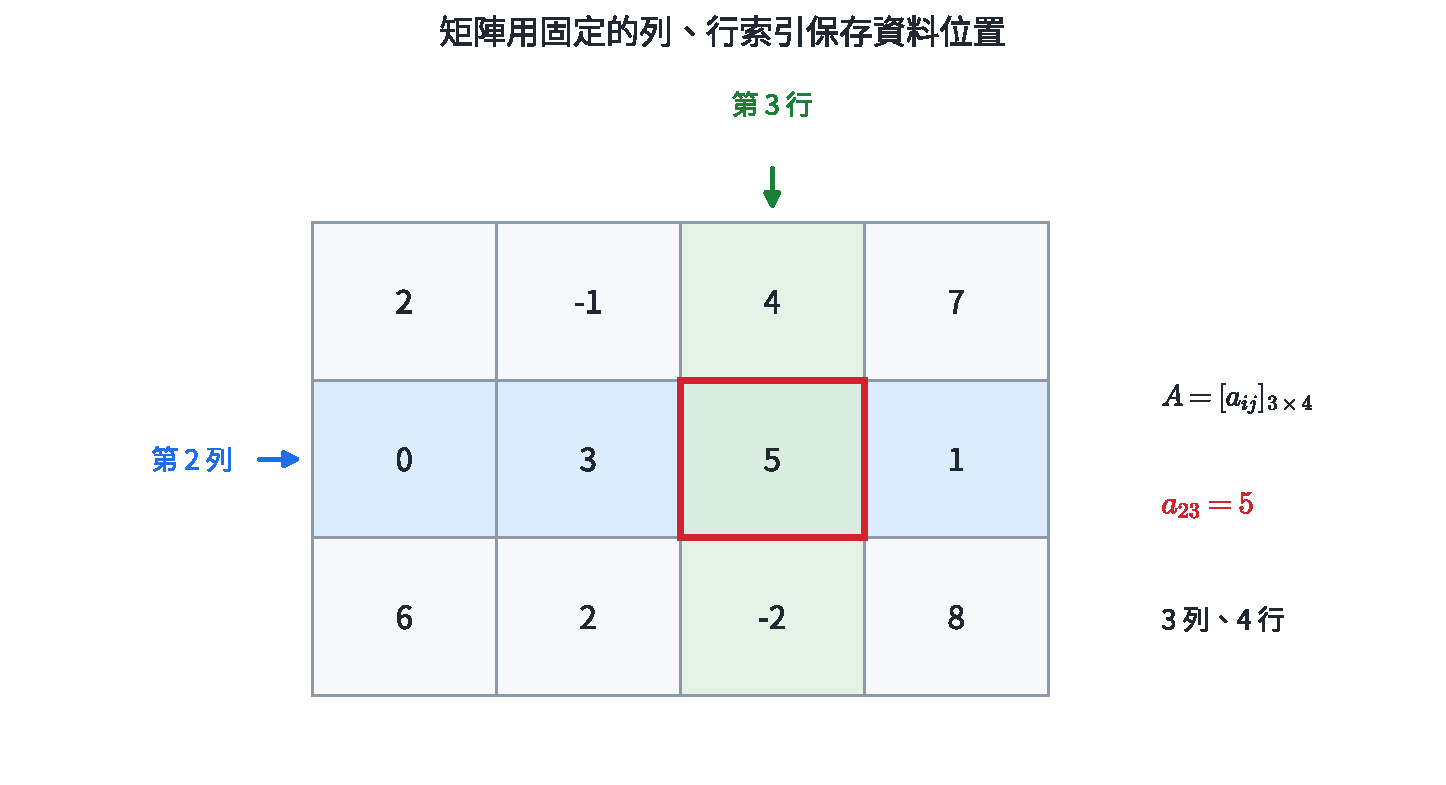
\includegraphics[width=0.86\linewidth,height=\textheight,keepaspectratio,alt={圖 4｜矩陣的列、行與元素位置；紅框元素位於第 2 列、第 3 行。}]{assets/數A4-4-列行與元素.pdf}
\caption{圖 4｜矩陣的列、行與元素位置；紅框元素位於第 2 列、第 3 行。}
\end{figure}

常用特殊矩陣包括：

\[
O_{m\times n}=
\begin{bmatrix}
0&\cdots&0\\
\vdots&&\vdots\\
0&\cdots&0
\end{bmatrix},
\]

以及主對角線為 \(1\)、其他元素為 \(0\) 的單位方陣 \(I_n\)。

\begin{HandoutWorkedExample}

\subsection{完整示範｜由索引規則建立矩陣}\label{ux5b8cux6574ux793aux7bc4ux7531ux7d22ux5f15ux898fux5247ux5efaux7acbux77e9ux9663}

已知 \(A=[a_{ij}]_{2\times3}\)，且 \(a_{ij}=2i-j\)。逐一代入 \(i=1,2\) 與 \(j=1,2,3\)：

\[
\begin{aligned}
(a_{11},a_{12},a_{13})&=(1,0,-1),\\
(a_{21},a_{22},a_{23})&=(3,2,1).
\end{aligned}
\]

所以

\[
\boxed{
A=
\begin{bmatrix}
1&0&-1\\
3&2&1
\end{bmatrix}}
\]

且 \(A\) 為 \(2\times3\) 階矩陣，\(a_{23}=1\)。

\end{HandoutWorkedExample}

\begin{HandoutWorkedExample}

\subsection{完整示範｜由矩陣相等求參數}\label{ux5b8cux6574ux793aux7bc4ux7531ux77e9ux9663ux76f8ux7b49ux6c42ux53c3ux6578}

若

\[
\begin{bmatrix}
x&2y\\
-1&x+y
\end{bmatrix}
=
\begin{bmatrix}
3&4\\
-1&5
\end{bmatrix},
\]

對應元素相等，得到

\[
x=3,\qquad 2y=4,\qquad x+y=5.
\]

前兩式給出 \(x=3,y=2\)，也滿足第三式。因此

\[
\boxed{x=3,\quad y=2}.
\]

\end{HandoutWorkedExample}

\subsection{2.2 加法、減法與係數積}\label{ux52a0ux6cd5ux6e1bux6cd5ux8207ux4fc2ux6578ux7a4d}

只有階數相同的矩陣能逐位置相加、相減：

\[
[a_{ij}]+[b_{ij}]=[a_{ij}+b_{ij}],
\]

\[
[a_{ij}]-[b_{ij}]=[a_{ij}-b_{ij}].
\]

實數 \(r\) 與矩陣相乘時，每個元素都乘 \(r\)：

\[
r[a_{ij}]=[ra_{ij}].
\]

若矩陣記錄同一套列、行索引，加法表示資料合併，減法表示逐項變化，係數積表示整批縮放。

\begin{HandoutWorkedExample}

\subsection{完整示範｜兩週資料合併與平均}\label{ux5b8cux6574ux793aux7bc4ux5169ux9031ux8cc7ux6599ux5408ux4f75ux8207ux5e73ux5747}

甲、乙兩門市兩週三項商品銷量為

\[
W_1=
\begin{bmatrix}
12&8&5\\
9&11&6
\end{bmatrix},\qquad
W_2=
\begin{bmatrix}
15&7&9\\
10&13&8
\end{bmatrix}.
\]

兩週合計為

\[
W_1+W_2
=
\boxed{
\begin{bmatrix}
27&15&14\\
19&24&14
\end{bmatrix}}.
\]

每週平均銷量矩陣為

\[
\frac12(W_1+W_2)
=
\boxed{
\begin{bmatrix}
13.5&7.5&7\\
9.5&12&7
\end{bmatrix}}.
\]

每個位置始終代表同一門市、同一商品，因此逐項運算具有一致資料意義。

\end{HandoutWorkedExample}

\begin{HandoutWorkedExample}

\subsection{完整示範｜解矩陣方程式}\label{ux5b8cux6574ux793aux7bc4ux89e3ux77e9ux9663ux65b9ux7a0bux5f0f}

已知

\[
A=
\begin{bmatrix}
2&-1\\
3&4
\end{bmatrix},\qquad
B=
\begin{bmatrix}
1&2\\
-2&5
\end{bmatrix},
\]

且 \(2X+A=3B\)。移項得

\[
2X=3B-A,\qquad X=\frac12(3B-A).
\]

\[
3B-A
=
\begin{bmatrix}
3&6\\
-6&15
\end{bmatrix}
-
\begin{bmatrix}
2&-1\\
3&4
\end{bmatrix}
=
\begin{bmatrix}
1&7\\
-9&11
\end{bmatrix}.
\]

所以

\[
\boxed{
X=
\begin{bmatrix}
\tfrac12&\tfrac72\\
-\tfrac92&\tfrac{11}{2}
\end{bmatrix}}.
\]

代回 \(2X+A\) 可逐項得到 \(3B\)。

\end{HandoutWorkedExample}

矩陣加法與係數積保留下列性質：

\[
A+B=B+A,\qquad (A+B)+C=A+(B+C),
\]

\[
r(A+B)=rA+rB,\qquad (r+s)A=rA+sA.
\]

這些性質可由每個第 \((i,j)\) 元的實數運算直接證明。

\begin{HandoutSelfCheck}

\subsection{分節練習｜矩陣索引與逐項運算}\label{ux5206ux7bc0ux7df4ux7fd2ux77e9ux9663ux7d22ux5f15ux8207ux9010ux9805ux904bux7b97}

\begin{enumerate}
\def\labelenumi{\arabic{enumi}.}
\tightlist
\item
  已知 \(A=[a_{ij}]_{3\times2}\)、\(a_{ij}=i+2j\)，寫出 \(A\) 並求 \(a_{31}\)。
\item
  若
  \[
  \begin{bmatrix}p&q-1\\2p&r\end{bmatrix}
  =
  \begin{bmatrix}2&4\\4&-3\end{bmatrix},
  \]
  求 \(p,q,r\)。
\item
  設
  \[
  A=\begin{bmatrix}1&-2\\3&0\end{bmatrix},
  \quad
  B=\begin{bmatrix}4&1\\-1&5\end{bmatrix},
  \]
  求 \(2A-B\)。
\item
  兩批同規格資料矩陣為
  \[
  D_1=\begin{bmatrix}8&12&10\\6&9&15\end{bmatrix},
  \quad
  D_2=\begin{bmatrix}4&5&8\\7&3&5\end{bmatrix}.
  \]
  求合計矩陣與第二批相對第一批的變化矩陣 \(D_2-D_1\)。
\item
  已知 \(3(X-A)=2B\)，其中
  \[
  A=\begin{bmatrix}1&0\\-1&2\end{bmatrix},
  \quad
  B=\begin{bmatrix}3&-3\\6&0\end{bmatrix},
  \]
  求 \(X\)。
\item
  說明為何 \(2\times3\) 矩陣與 \(3\times2\) 矩陣無法相加。
\end{enumerate}

\textbf{解答}

\begin{enumerate}
\def\labelenumi{\arabic{enumi}.}
\tightlist
\item
  \(\boxed{A=\begin{bmatrix}3&5\\4&6\\5&7\end{bmatrix}}\)，且 \(\boxed{a_{31}=5}\)。
\item
  對應元素相等得 \(\boxed{p=2,q=5,r=-3}\)。
\item
  \(\boxed{2A-B=\begin{bmatrix}-2&-5\\7&-5\end{bmatrix}}\)。
\item
  合計為 \(\boxed{\begin{bmatrix}12&17&18\\13&12&20\end{bmatrix}}\)；變化為 \(\boxed{\begin{bmatrix}-4&-7&-2\\1&-6&-10\end{bmatrix}}\)。
\item
  \(X=A+\frac23B\)，所以 \(\boxed{X=\begin{bmatrix}3&-2\\3&2\end{bmatrix}}\)。
\item
  加法要讓每個第 \((i,j)\) 元都有同位置的配對；兩矩陣列數與行數不同，位置集合不同。
\end{enumerate}

\end{HandoutSelfCheck}

\section{3. 矩陣乘法、運算順序與資料組合}\label{ux77e9ux9663ux4e58ux6cd5ux904bux7b97ux9806ux5e8fux8207ux8cc7ux6599ux7d44ux5408}

\subsection{3.1 列乘行的定義}\label{ux5217ux4e58ux884cux7684ux5b9aux7fa9}

設 \(A=[a_{ij}]\) 是 \(m\times n\) 矩陣，\(B=[b_{jk}]\) 是 \(n\times p\) 矩陣。兩者相接的維度同為 \(n\)，乘積 \(AB\) 定義為 \(m\times p\) 矩陣，且

\[
(AB)_{ik}=\sum_{j=1}^{n}a_{ij}b_{jk}.
\]

第 \((i,k)\) 元由 \(A\) 的第 \(i\) 列與 \(B\) 的第 \(k\) 行逐項相乘後加總。共享索引 \(j\) 被加總，外側索引 \(i,k\) 保留下來：

\[
\underbrace{(m\times n)}_{A}
\underbrace{(n\times p)}_{B}
\longrightarrow
\underbrace{(m\times p)}_{AB}.
\]

\begin{figure}
\centering
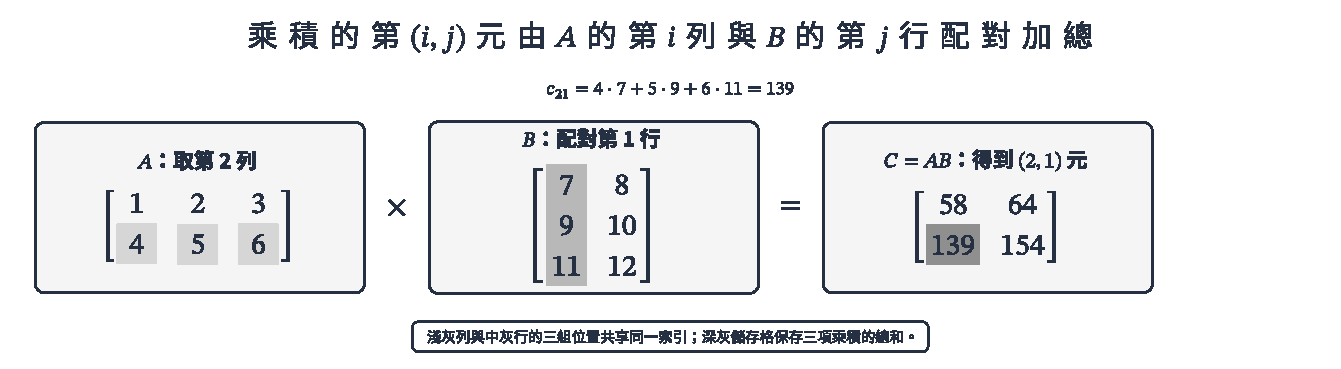
\includegraphics[width=0.94\linewidth,height=\textheight,keepaspectratio,alt={圖 5｜乘積的一個元素由左矩陣的一列與右矩陣的一行配對；共享索引的三項乘積相加。}]{assets/數A4-4-列乘行.pdf}
\caption{圖 5｜乘積的一個元素由左矩陣的一列與右矩陣的一行配對；共享索引的三項乘積相加。}
\end{figure}

\begin{HandoutWorkedExample}

\subsection{完整示範｜計算非方陣的乘積}\label{ux5b8cux6574ux793aux7bc4ux8a08ux7b97ux975eux65b9ux9663ux7684ux4e58ux7a4d}

設

\[
A=
\begin{bmatrix}
1&2&3\\
4&5&6
\end{bmatrix},
\qquad
B=
\begin{bmatrix}
7&8\\
9&10\\
11&12
\end{bmatrix}.
\]

\(A\) 是 \(2\times3\)，\(B\) 是 \(3\times2\)，所以 \(AB\) 存在且為 \(2\times2\)：

\[
AB=
\begin{bmatrix}
1\cdot7+2\cdot9+3\cdot11&
1\cdot8+2\cdot10+3\cdot12\\
4\cdot7+5\cdot9+6\cdot11&
4\cdot8+5\cdot10+6\cdot12
\end{bmatrix}
=
\boxed{
\begin{bmatrix}
58&64\\
139&154
\end{bmatrix}}.
\]

四個答案分別使用不同的「列---行」配對。

\end{HandoutWorkedExample}

\begin{HandoutWorkedExample}

\subsection{完整示範｜先由階數判斷運算是否合法}\label{ux5b8cux6574ux793aux7bc4ux5148ux7531ux968eux6578ux5224ux65b7ux904bux7b97ux662fux5426ux5408ux6cd5}

若 \(C\) 為 \(3\times2\)、\(D\) 為 \(2\times4\)，則

\[
CD:(3\times2)(2\times4)\longrightarrow3\times4.
\]

\(DC\) 需要把 \(D\) 的行數 \(4\) 與 \(C\) 的列數 \(3\) 接合，兩者不同，所以 \(DC\) 沒有定義。矩陣乘法的順序同時決定運算是否存在與結果的階數。

\end{HandoutWorkedExample}

\subsection{3.2 乘法性質與運算順序}\label{ux4e58ux6cd5ux6027ux8ceaux8207ux904bux7b97ux9806ux5e8f}

合適階數下，矩陣乘法滿足

\[
(AB)C=A(BC),\qquad A(B+C)=AB+AC,\qquad (A+B)C=AC+BC.
\]

單位方陣 \(I_n\) 在乘法中保留原矩陣：

\[
I_mA=A=AI_n
\]

其中 \(A\) 為 \(m\times n\)。結合律來自有限和式可重新分組：

\[
\bigl((AB)C\bigr)_{i\ell}
=\sum_k\left(\sum_j a_{ij}b_{jk}\right)c_{k\ell}
=\sum_j a_{ij}\left(\sum_k b_{jk}c_{k\ell}\right)
=\bigl(A(BC)\bigr)_{i\ell}.
\]

矩陣乘法通常不具交換律，因為左側矩陣決定輸出列，右側矩陣決定輸出行；交換順序會改變配對與作用次序。

\begin{HandoutWorkedExample}

\subsection{完整示範｜同一組矩陣的兩種順序}\label{ux5b8cux6574ux793aux7bc4ux540cux4e00ux7d44ux77e9ux9663ux7684ux5169ux7a2eux9806ux5e8f}

設

\[
A=\begin{bmatrix}1&1\\0&1\end{bmatrix},
\qquad
B=\begin{bmatrix}1&0\\1&1\end{bmatrix}.
\]

直接計算得

\[
AB=\begin{bmatrix}2&1\\1&1\end{bmatrix},
\qquad
BA=\begin{bmatrix}1&1\\1&2\end{bmatrix}.
\]

因此 \(AB\ne BA\)。若兩矩陣代表連續兩次資料處理，右側的規則先作用；改成另一個乘積就代表改變處理順序。

\end{HandoutWorkedExample}

\begin{HandoutWorkedExample}

\subsection{完整示範｜非零矩陣的乘積可以是零矩陣}\label{ux5b8cux6574ux793aux7bc4ux975eux96f6ux77e9ux9663ux7684ux4e58ux7a4dux53efux4ee5ux662fux96f6ux77e9ux9663}

令

\[
A=\begin{bmatrix}1&0\\0&0\end{bmatrix},
\qquad
B=\begin{bmatrix}0&0\\0&1\end{bmatrix}.
\]

\(A\) 保留向量的第一分量，\(B\) 的輸出只可能出現在第二分量。兩個規則依序作用時，

\[
AB=
\begin{bmatrix}0&0\\0&0\end{bmatrix}.
\]

\(A\) 與 \(B\) 都是非零矩陣，仍有 \(AB=O\)，因此 \(A\) 與 \(B\) 都是零因子。矩陣消去律需要額外的可逆條件。

\end{HandoutWorkedExample}

\subsection{3.3 數量、單價與影像資料}\label{ux6578ux91cfux55aeux50f9ux8207ux5f71ux50cfux8cc7ux6599}

矩陣乘法的共享索引常代表「同一類別」。若 \(Q\) 的列表示門市、行表示商品，\(P\) 的列表示商品、行表示月份，則

\[
(QP)_{\text{門市,月份}}
=\sum_{\text{商品}}
(\text{數量})(\text{單價}),
\]

正是各門市各月份的總成本。索引的語意能判斷乘法順序是否合理。

\begin{figure}
\centering
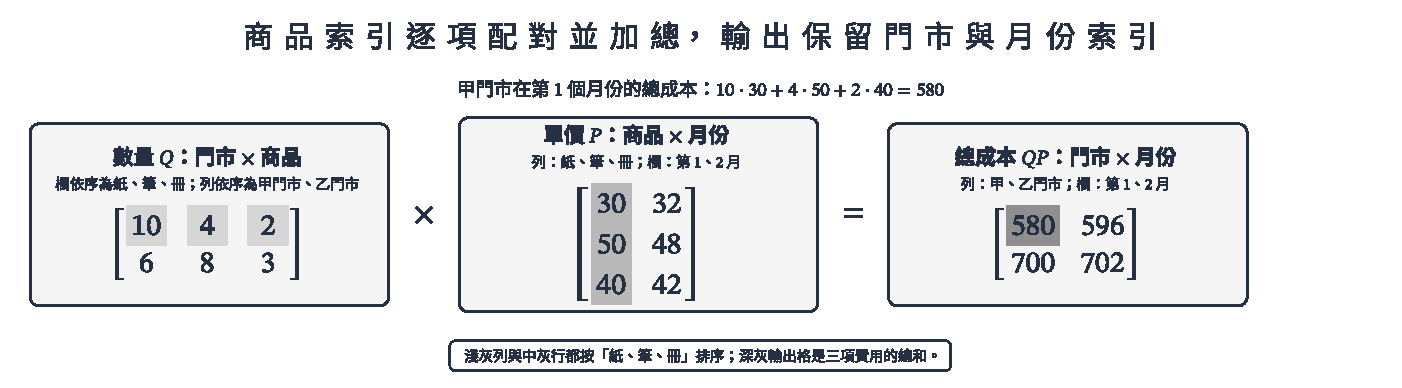
\includegraphics[width=0.96\linewidth,height=\textheight,keepaspectratio,alt={圖 6｜商品索引在數量矩陣與單價矩陣中配對並加總，輸出保留門市與月份。}]{assets/數A4-4-資料表乘法.pdf}
\caption{圖 6｜商品索引在數量矩陣與單價矩陣中配對並加總，輸出保留門市與月份。}
\end{figure}

\begin{HandoutWorkedExample}

\subsection{完整示範｜兩家門市、三類商品、兩個月份}\label{ux5b8cux6574ux793aux7bc4ux5169ux5bb6ux9580ux5e02ux4e09ux985eux5546ux54c1ux5169ux500bux6708ux4efd}

兩家門市的商品數量為

\[
Q=
\begin{bmatrix}
10&4&2\\
6&8&3
\end{bmatrix},
\]

三類商品在兩個月份的單價為

\[
P=
\begin{bmatrix}
30&32\\
50&48\\
40&42
\end{bmatrix}.
\]

總成本矩陣為

\[
QP=
\begin{bmatrix}
10(30)+4(50)+2(40)&10(32)+4(48)+2(42)\\
6(30)+8(50)+3(40)&6(32)+8(48)+3(42)
\end{bmatrix}
=
\boxed{\begin{bmatrix}580&596\\700&702\end{bmatrix}}.
\]

例如右下角 \(702\) 表示第二家門市在第二個月份的總成本。

\end{HandoutWorkedExample}

\clearpage

\begin{HandoutWorkedExample}

\subsection{完整示範｜用矩陣調整兩通道影像}\label{ux5b8cux6574ux793aux7bc4ux7528ux77e9ux9663ux8abfux6574ux5169ux901aux9053ux5f71ux50cf}

一個像素的兩個通道寫成

\[
v=\begin{bmatrix}120\\80\end{bmatrix}.
\]

處理矩陣

\[
C=\begin{bmatrix}0.8&0.1\\0.2&0.9\end{bmatrix}
\]

把舊通道混合成新通道：

\[
Cv=
\begin{bmatrix}
0.8(120)+0.1(80)\\
0.2(120)+0.9(80)
\end{bmatrix}
=\boxed{\begin{bmatrix}104\\96\end{bmatrix}}.
\]

每一列是一個新通道的配方。大量像素可排成資料矩陣，一次套用相同規則。

\end{HandoutWorkedExample}

\begin{HandoutSelfCheck}

\subsection{分節練習｜矩陣乘法與資料組合}\label{ux5206ux7bc0ux7df4ux7fd2ux77e9ux9663ux4e58ux6cd5ux8207ux8cc7ux6599ux7d44ux5408}

\begin{enumerate}
\def\labelenumi{\arabic{enumi}.}
\tightlist
\item
  設 \(A=\begin{bmatrix}2&-1&3\\0&4&1\end{bmatrix}\)、\(B=\begin{bmatrix}1&2\\3&0\\-2&5\end{bmatrix}\)，求 \(AB\)。
\item
  \(M\) 為 \(4\times3\)、\(N\) 為 \(3\times5\)、\(P\) 為 \(5\times2\)。寫出 \(MN\)、\(NP\)、\(MNP\) 的階數。
\item
  設 \(A=\begin{bmatrix}1&2\\0&1\end{bmatrix}\)、\(B=\begin{bmatrix}2&0\\1&3\end{bmatrix}\)，分別求 \(AB\) 與 \(BA\)。
\item
  求矩陣 \(X\)，使 \(\begin{bmatrix}1&2\\3&4\end{bmatrix}X=\begin{bmatrix}2&1\\4&3\end{bmatrix}\)，也就是交換兩個直行。
\item
  一家工廠生產甲、乙兩型產品，每件分別需材料 \((2,1,3)\) 與 \((1,4,2)\) 單位；三種材料單價為 \((30,20,10)\) 元。用矩陣乘法求兩型產品的材料成本。
\item
  三個像素的兩通道資料排列成 \(D=\begin{bmatrix}100&60&20\\40&80&120\end{bmatrix}\)，其中每個直行代表一個像素。若 \(C=\begin{bmatrix}1&0\\0.25&0.75\end{bmatrix}\)，求 \(CD\)，並說明第一通道是否改變。
\end{enumerate}

\textbf{解答}

\begin{enumerate}
\def\labelenumi{\arabic{enumi}.}
\tightlist
\item
  \(\boxed{AB=\begin{bmatrix}-7&19\\10&5\end{bmatrix}}\)。
\item
  \(MN\) 為 \(\boxed{4\times5}\)，\(NP\) 為 \(\boxed{3\times2}\)，\(MNP\) 為 \(\boxed{4\times2}\)。
\item
  \(\boxed{AB=\begin{bmatrix}4&6\\1&3\end{bmatrix}}\)，\(\boxed{BA=\begin{bmatrix}2&4\\1&5\end{bmatrix}}\)。
\item
  右乘交換矩陣即可交換兩個直行，故 \(\boxed{X=\begin{bmatrix}0&1\\1&0\end{bmatrix}}\)；相乘後確為 \(\begin{bmatrix}2&1\\4&3\end{bmatrix}\)。
\item
  \(\begin{bmatrix}2&1&3\\1&4&2\end{bmatrix}\begin{bmatrix}30\\20\\10\end{bmatrix}=\boxed{\begin{bmatrix}110\\130\end{bmatrix}}\) 元。
\item
  \(\boxed{CD=\begin{bmatrix}100&60&20\\55&75&95\end{bmatrix}}\)；\(C\) 的第一列為 \((1,0)\)，所以第一通道保留原值。
\end{enumerate}

\end{HandoutSelfCheck}

\section{4. 行列式、反方陣與矩陣方程式}\label{ux884cux5217ux5f0fux53cdux65b9ux9663ux8207ux77e9ux9663ux65b9ux7a0bux5f0f}

\subsection{4.1 二階行列式與面積倍率}\label{ux4e8cux968eux884cux5217ux5f0fux8207ux9762ux7a4dux500dux7387}

二階方陣

\[
A=\begin{bmatrix}a&b\\c&d\end{bmatrix}
\]

的行列式定義為

\[
\det A=ad-bc.
\]

\(A\) 的兩個直行向量為 \(u=(a,c)\)、\(v=(b,d)\)。由它們張成的平行四邊形，有向面積為 \(ad-bc\)，實際面積為

\[
\boxed{|\det A|}.
\]

當 \(\det A=0\)，兩個直行向量線性相依，平面被壓到一條線或一個點；不同輸入可能得到相同輸出，復原結果不唯一。

\begin{figure}
\centering
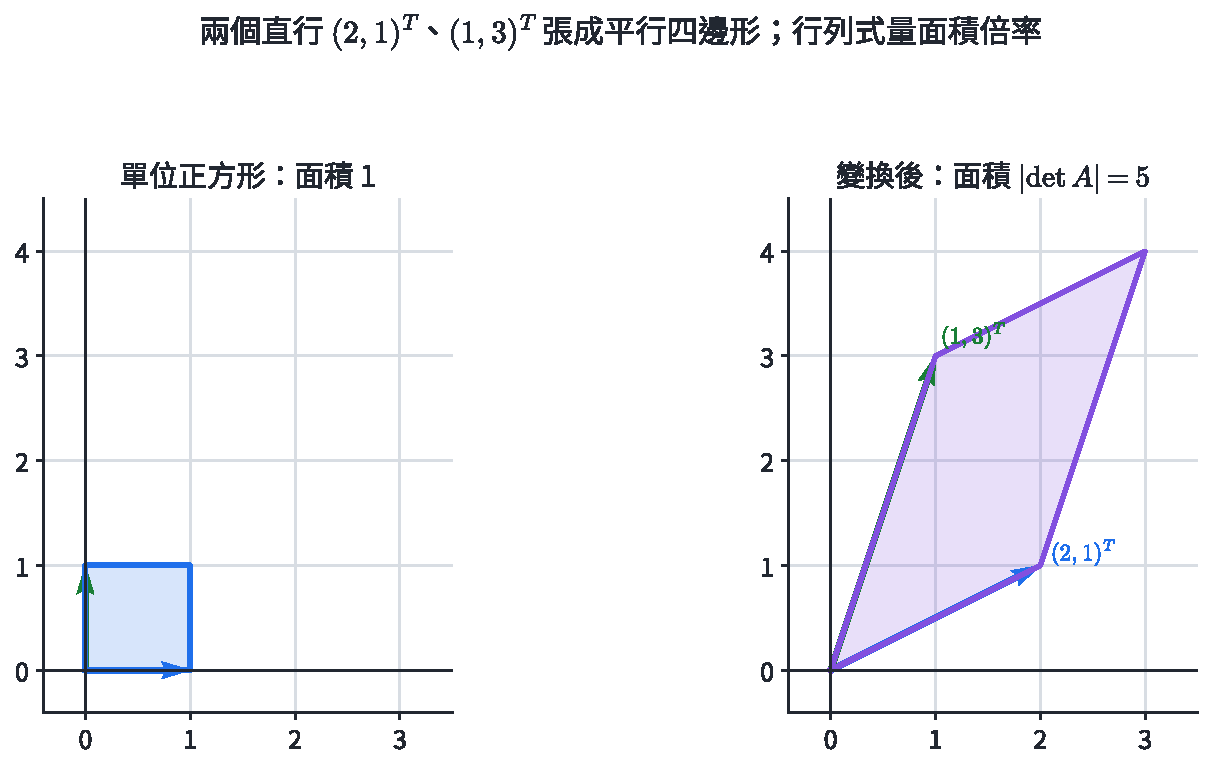
\includegraphics[width=0.92\linewidth,height=\textheight,keepaspectratio,alt={圖 7｜二階矩陣的兩個直行張成平行四邊形，面積倍率是行列式絕對值。}]{assets/數A4-4-行列式與面積.pdf}
\caption{圖 7｜二階矩陣的兩個直行張成平行四邊形，面積倍率是行列式絕對值。}
\end{figure}

\begin{HandoutWorkedExample}

\subsection{完整示範｜由兩個輸出基底求面積}\label{ux5b8cux6574ux793aux7bc4ux7531ux5169ux500bux8f38ux51faux57faux5e95ux6c42ux9762ux7a4d}

矩陣

\[
A=\begin{bmatrix}3&1\\1&2\end{bmatrix}
\]

把標準正方形的兩條邊變成 \((3,1)\) 與 \((1,2)\)。平行四邊形面積為

\[
|\det A|=|3\cdot2-1\cdot1|=\boxed{5}.
\]

因此任何圖形經此線性變換後，面積都變成原來的 \(5\) 倍。

\end{HandoutWorkedExample}

\begin{HandoutWorkedExample}

\subsection{完整示範｜參數控制面積是否塌縮}\label{ux5b8cux6574ux793aux7bc4ux53c3ux6578ux63a7ux5236ux9762ux7a4dux662fux5426ux584cux7e2e}

設

\[
A_k=\begin{bmatrix}k&2\\3&k-1\end{bmatrix}.
\]

其行列式為

\[
\det A_k=k(k-1)-6=k^2-k-6=(k-3)(k+2).
\]

當 \(k=3\) 或 \(k=-2\)，面積倍率為 \(0\)，變換塌縮到一條線；其餘 \(k\) 值的面積倍率為 \(|(k-3)(k+2)|\)。

\end{HandoutWorkedExample}

\subsection{4.2 反方陣公式的推導}\label{ux53cdux65b9ux9663ux516cux5f0fux7684ux63a8ux5c0e}

若存在矩陣 \(A^{-1}\) 使

\[
AA^{-1}=A^{-1}A=I,
\]

則稱 \(A\) 可逆，\(A^{-1}\) 稱為 \(A\) 的反方陣。對二階方陣，先觀察

\[
\begin{bmatrix}a&b\\c&d\end{bmatrix}
\begin{bmatrix}d&-b\\-c&a\end{bmatrix}
=
\begin{bmatrix}ad-bc&0\\0&ad-bc\end{bmatrix}
=(\det A)I.
\]

只要 \(\det A\ne0\)，兩側除以 \(\det A\)，得到

\[
\boxed{
A^{-1}=\frac1{ad-bc}
\begin{bmatrix}d&-b\\-c&a\end{bmatrix}}.
\]

\begin{figure}
\centering
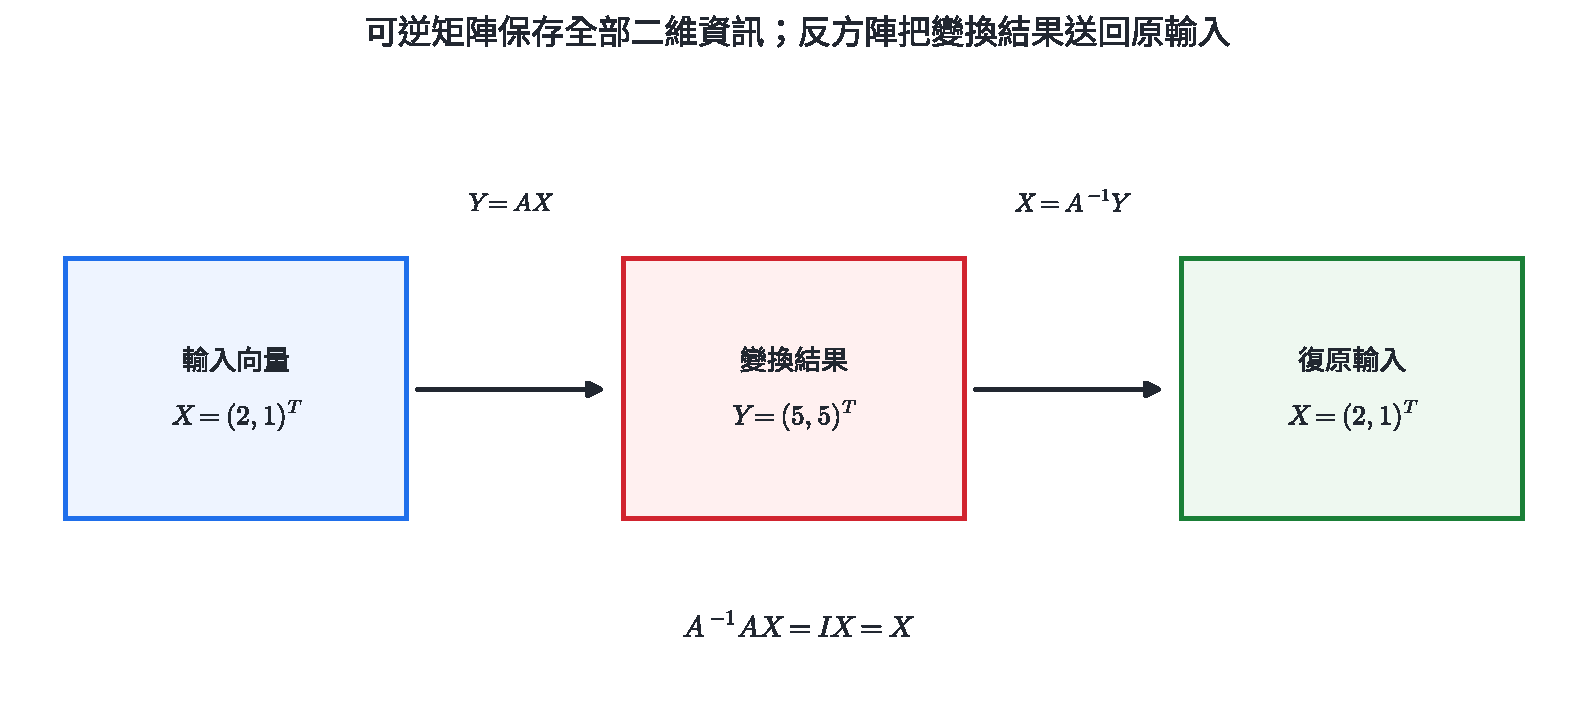
\includegraphics[width=0.94\linewidth,height=\textheight,keepaspectratio,alt={圖 8｜可逆矩陣先改變坐標，再由反方陣把每個輸出唯一送回原輸入。}]{assets/數A4-4-反方陣復原.pdf}
\caption{圖 8｜可逆矩陣先改變坐標，再由反方陣把每個輸出唯一送回原輸入。}
\end{figure}

\clearpage

\begin{HandoutWorkedExample}

\subsection{完整示範｜計算反方陣並雙向驗算}\label{ux5b8cux6574ux793aux7bc4ux8a08ux7b97ux53cdux65b9ux9663ux4e26ux96d9ux5411ux9a57ux7b97}

設

\[
A=\begin{bmatrix}2&1\\1&3\end{bmatrix}.
\]

\(\det A=6-1=5\)，所以

\[
A^{-1}=\frac15\begin{bmatrix}3&-1\\-1&2\end{bmatrix}.
\]

驗算：

\[
AA^{-1}
=\frac15
\begin{bmatrix}
6-1&-2+2\\
3-3&-1+6
\end{bmatrix}
=I.
\]

同理可得 \(A^{-1}A=I\)。

\end{HandoutWorkedExample}

\begin{HandoutWorkedExample}

\subsection{完整示範｜乘積的反方陣順序}\label{ux5b8cux6574ux793aux7bc4ux4e58ux7a4dux7684ux53cdux65b9ux9663ux9806ux5e8f}

若 \(A,B\) 都可逆，則

\[
(AB)(B^{-1}A^{-1})
=A(BB^{-1})A^{-1}
=I.
\]

另一側也有

\[
(B^{-1}A^{-1})(AB)
=B^{-1}(A^{-1}A)B
=I.
\]

因此

\[
\boxed{(AB)^{-1}=B^{-1}A^{-1}}.
\]

逆運算按相反順序撤銷：先撤銷最後作用的 \(A\)，再撤銷先前作用的 \(B\)。

\end{HandoutWorkedExample}

\subsection{4.3 用反方陣解向量與矩陣方程式}\label{ux7528ux53cdux65b9ux9663ux89e3ux5411ux91cfux8207ux77e9ux9663ux65b9ux7a0bux5f0f}

若 \(Ax=b\) 且 \(A\) 可逆，左乘 \(A^{-1}\) 得

\[
x=A^{-1}b.
\]

若未知矩陣位在乘積左側，例如 \(XA=B\)，則需右乘 \(A^{-1}\)：

\[
X=BA^{-1}.
\]

乘在哪一側由未知矩陣的位置決定；等式兩側需保留相同的矩陣順序。

\begin{HandoutWorkedExample}

\subsection{完整示範｜由混合後資料復原原始量}\label{ux5b8cux6574ux793aux7bc4ux7531ux6df7ux5408ux5f8cux8cc7ux6599ux5fa9ux539fux539fux59cbux91cf}

已知

\[
\begin{bmatrix}2&1\\1&3\end{bmatrix}
\begin{bmatrix}x\\y\end{bmatrix}
=
\begin{bmatrix}5\\5\end{bmatrix}.
\]

使用前例反方陣：

\[
\begin{bmatrix}x\\y\end{bmatrix}
=\frac15
\begin{bmatrix}3&-1\\-1&2\end{bmatrix}
\begin{bmatrix}5\\5\end{bmatrix}
=\frac15\begin{bmatrix}10\\5\end{bmatrix}
=\boxed{\begin{bmatrix}2\\1\end{bmatrix}}.
\]

代回左側得 \((5,5)^T\)。

\end{HandoutWorkedExample}

\begin{HandoutWorkedExample}

\subsection{完整示範｜未知矩陣位在乘積左側}\label{ux5b8cux6574ux793aux7bc4ux672aux77e5ux77e9ux9663ux4f4dux5728ux4e58ux7a4dux5de6ux5074}

解

\[
X
\begin{bmatrix}1&2\\0&1\end{bmatrix}
=
\begin{bmatrix}3&8\\2&5\end{bmatrix}.
\]

令

\[
A=\begin{bmatrix}1&2\\0&1\end{bmatrix},
\qquad
A^{-1}=\begin{bmatrix}1&-2\\0&1\end{bmatrix}.
\]

在等式右側乘 \(A^{-1}\)：

\[
X=
\begin{bmatrix}3&8\\2&5\end{bmatrix}
\begin{bmatrix}1&-2\\0&1\end{bmatrix}
=
\boxed{\begin{bmatrix}3&2\\2&1\end{bmatrix}}.
\]

驗算 \(XA\) 可還原題目的右側矩陣。

\end{HandoutWorkedExample}

\begin{HandoutSelfCheck}

\subsection{分節練習｜行列式、反方陣與方程式}\label{ux5206ux7bc0ux7df4ux7fd2ux884cux5217ux5f0fux53cdux65b9ux9663ux8207ux65b9ux7a0bux5f0f}

\begin{enumerate}
\def\labelenumi{\arabic{enumi}.}
\tightlist
\item
  求 \(A=\begin{bmatrix}4&-1\\2&3\end{bmatrix}\) 的行列式與反方陣。
\item
  求 \(k\) 的範圍，使 \(\begin{bmatrix}k&1\\4&k\end{bmatrix}\) 可逆。
\item
  一個三角形面積為 \(6\)，經矩陣 \(\begin{bmatrix}2&1\\-1&3\end{bmatrix}\) 變換後，求新面積。
\item
  解 \(\begin{bmatrix}3&1\\1&2\end{bmatrix}\begin{bmatrix}x\\y\end{bmatrix}=\begin{bmatrix}5\\5\end{bmatrix}\)。
\item
  解 \(AX=B\)，其中 \(A=\begin{bmatrix}2&0\\1&1\end{bmatrix}\)、\(B=\begin{bmatrix}4&2\\3&5\end{bmatrix}\)。
\item
  已知 \(A,B\) 均可逆，化簡 \((A^{-1}B)^{-1}\)，並以乘法驗證。
\end{enumerate}

\textbf{解答}

\begin{enumerate}
\def\labelenumi{\arabic{enumi}.}
\tightlist
\item
  \(\det A=14\)，\(\boxed{A^{-1}=\frac1{14}\begin{bmatrix}3&1\\-2&4\end{bmatrix}}\)。
\item
  行列式為 \(k^2-4\)；可逆條件為 \(\boxed{k\ne2,-2}\)。
\item
  面積倍率為 \(|2(3)-1(-1)|=7\)，新面積為 \(\boxed{42}\)。
\item
  反方陣為 \(\frac15\begin{bmatrix}2&-1\\-1&3\end{bmatrix}\)，故 \(\boxed{(x,y)=(1,2)}\)。
\item
  \(X=A^{-1}B\)，\(A^{-1}=\begin{bmatrix}\tfrac12&0\\-\tfrac12&1\end{bmatrix}\)，所以 \(\boxed{X=\begin{bmatrix}2&1\\1&4\end{bmatrix}}\)。
\item
  \(\boxed{(A^{-1}B)^{-1}=B^{-1}A}\)；\((A^{-1}B)(B^{-1}A)=I\)，反向乘法也為 \(I\)。
\end{enumerate}

\end{HandoutSelfCheck}

\section{5. 轉移矩陣與多期狀態}\label{ux8f49ux79fbux77e9ux9663ux8207ux591aux671fux72c0ux614b}

\subsection{5.1 狀態向量與轉移規則}\label{ux72c0ux614bux5411ux91cfux8207ux8f49ux79fbux898fux5247}

把第 \(n\) 期各狀態的比例排成直行向量

\[
X_n=\begin{bmatrix}x_{1,n}\\x_{2,n}\\\vdots\\x_{k,n}\end{bmatrix},
\qquad
x_{i,n}\ge0,\qquad
\sum_i x_{i,n}=1.
\]

若每一期都遵守同一套流動比例，令 \(a_{ij}\) 表示「目前在狀態 \(j\) 的量，下一期有多少比例進入狀態 \(i\)」，則

\[
X_{n+1}=AX_n,
\qquad
A=[a_{ij}].
\]

\(A\) 的每個直行描述一個原狀態的去向，因此每個直行的元素和為 \(1\)，且所有元素非負。這類矩陣稱為轉移矩陣。矩陣乘法會自動把不同來源流入同一狀態的量加總。

\begin{figure}
\centering
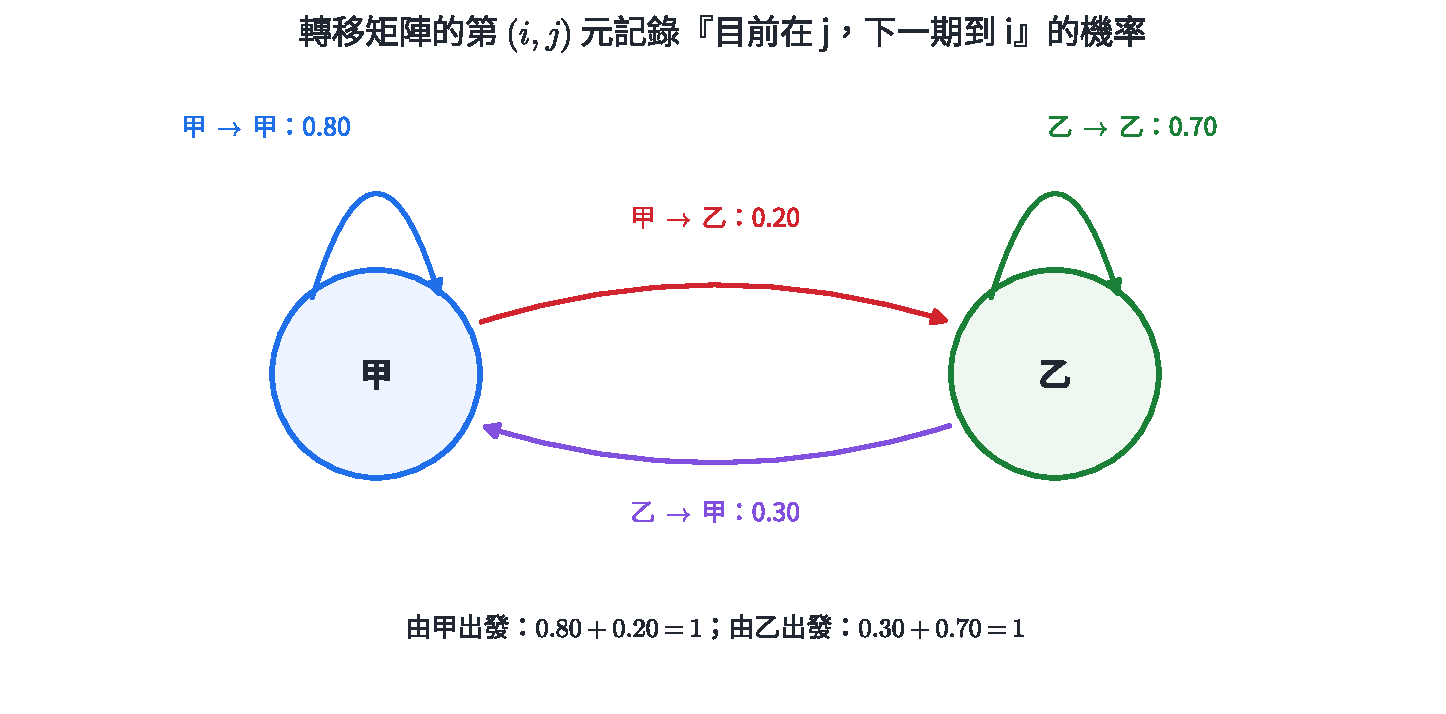
\includegraphics[width=0.92\linewidth,height=\textheight,keepaspectratio,alt={圖 9｜兩狀態轉移圖的每支箭頭對應矩陣的一個元素；每個原狀態的所有去向比例相加為 1。}]{assets/數A4-4-轉移狀態圖.pdf}
\caption{圖 9｜兩狀態轉移圖的每支箭頭對應矩陣的一個元素；每個原狀態的所有去向比例相加為 1。}
\end{figure}

\begin{HandoutWorkedExample}

\subsection{完整示範｜由轉移敘述建立矩陣}\label{ux5b8cux6574ux793aux7bc4ux7531ux8f49ux79fbux6558ux8ff0ux5efaux7acbux77e9ux9663}

某區域人口分成甲、乙兩區。每期甲區有 \(80\%\) 留在甲、\(20\%\) 前往乙；乙區有 \(30\%\) 前往甲、\(70\%\) 留在乙。以 \((\text{甲},\text{乙})\) 排列，轉移矩陣為

\[
A=
\begin{bmatrix}
0.8&0.3\\
0.2&0.7
\end{bmatrix}.
\]

第一個直行 \((0.8,0.2)^T\) 是甲區人口的去向；第二個直行 \((0.3,0.7)^T\) 是乙區人口的去向。若目前比例為

\[
X_0=\begin{bmatrix}0.9\\0.1\end{bmatrix},
\]

則下一期

\[
X_1=AX_0
=
\begin{bmatrix}
0.8(0.9)+0.3(0.1)\\
0.2(0.9)+0.7(0.1)
\end{bmatrix}
=\boxed{\begin{bmatrix}0.75\\0.25\end{bmatrix}}.
\]

兩分量仍非負且總和為 \(1\)。

\end{HandoutWorkedExample}

\begin{HandoutWorkedExample}

\subsection{完整示範｜連續兩期與矩陣冪}\label{ux5b8cux6574ux793aux7bc4ux9023ux7e8cux5169ux671fux8207ux77e9ux9663ux51aa}

沿用前例，

\[
X_2=AX_1=A(AX_0)=A^2X_0.
\]

因此

\[
X_2=
\begin{bmatrix}
0.8(0.75)+0.3(0.25)\\
0.2(0.75)+0.7(0.25)
\end{bmatrix}
=\boxed{\begin{bmatrix}0.675\\0.325\end{bmatrix}}.
\]

一般地，

\[
\boxed{X_n=A^nX_0}.
\]

矩陣冪表示同一轉移規則重複作用；\(A^n\) 的元素由連續的列乘行運算決定。

\end{HandoutWorkedExample}

\subsection{5.2 穩定狀態與參數估計}\label{ux7a69ux5b9aux72c0ux614bux8207ux53c3ux6578ux4f30ux8a08}

若某個比例向量 \(X_*\) 經一次轉移後保持不變，則

\[
AX_*=X_*,
\qquad
\sum_i (X_*)_i=1.
\]

這稱為穩定狀態。求解時把 \(AX_*=X_*\) 化成聯立方程式，再加入總和為 \(1\) 的條件。穩定狀態描述模型長期可能接近的固定比例；實際是否接近還要由轉移規則與初始狀態判斷。

\begin{figure}
\centering
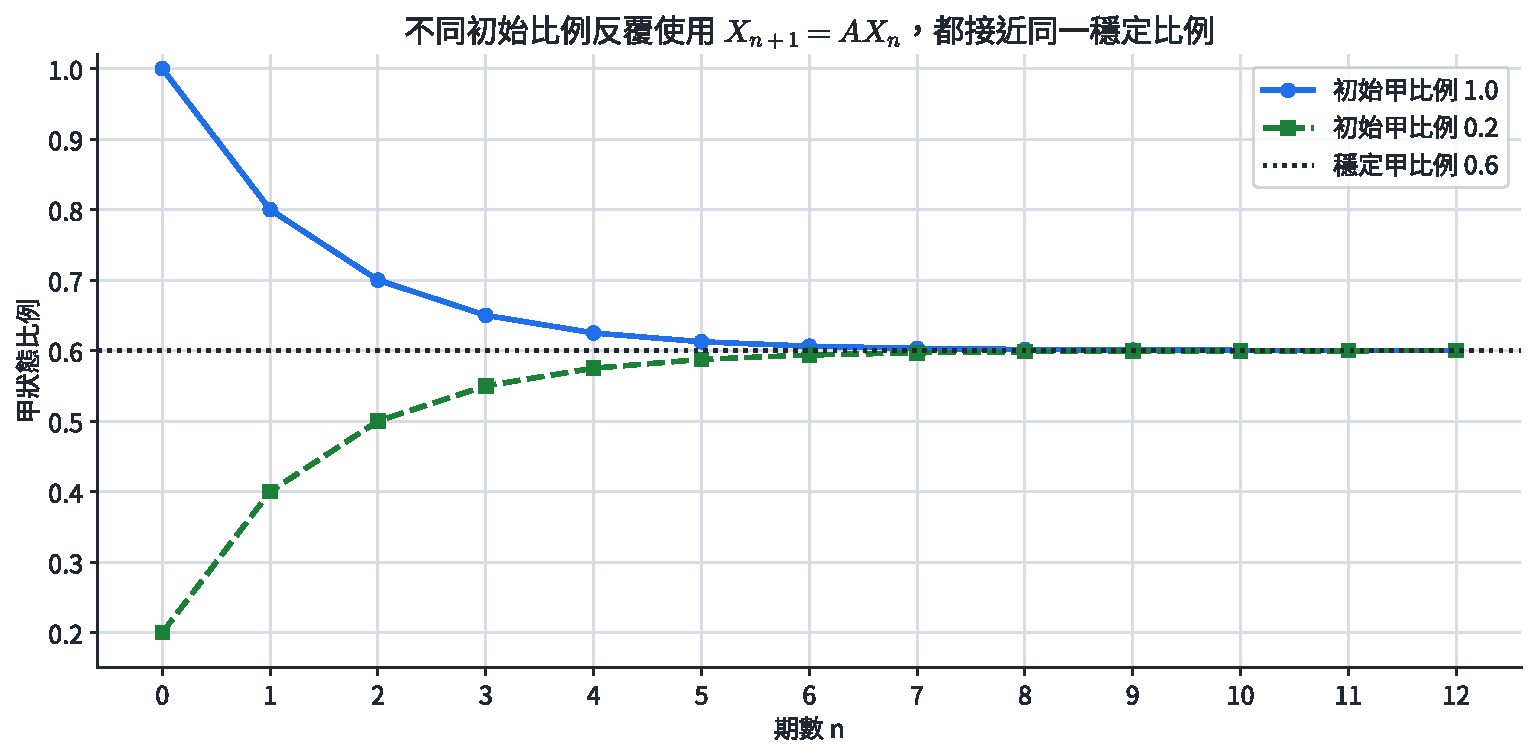
\includegraphics[width=0.94\linewidth,height=\textheight,keepaspectratio,alt={圖 10｜同一轉移矩陣從兩組不同初始比例反覆作用，甲狀態比例都逐期接近 0.6；乙狀態比例為 1-p\_n(\textbackslash text\{甲\})。}]{assets/數A4-4-轉移長期趨勢.pdf}
\caption{圖 10｜同一轉移矩陣從兩組不同初始比例反覆作用，甲狀態比例都逐期接近 0.6；乙狀態比例為 \(1-p_n(\text{甲})\)。}
\end{figure}

\begin{HandoutWorkedExample}

\subsection{完整示範｜解兩狀態穩定比例}\label{ux5b8cux6574ux793aux7bc4ux89e3ux5169ux72c0ux614bux7a69ux5b9aux6bd4ux4f8b}

對

\[
A=
\begin{bmatrix}
0.8&0.3\\
0.2&0.7
\end{bmatrix},
\qquad
X_*=\begin{bmatrix}x\\y\end{bmatrix},
\]

\(AX_*=X_*\) 的第一式為

\[
0.8x+0.3y=x
\quad\Longrightarrow\quad
0.2x=0.3y
\quad\Longrightarrow\quad
x:y=3:2.
\]

再用 \(x+y=1\)，得到

\[
\boxed{X_*=\begin{bmatrix}0.6\\0.4\end{bmatrix}}.
\]

驗算：

\[
A\begin{bmatrix}0.6\\0.4\end{bmatrix}
=
\begin{bmatrix}0.48+0.12\\0.12+0.28\end{bmatrix}
=
\begin{bmatrix}0.6\\0.4\end{bmatrix}.
\]

\end{HandoutWorkedExample}

\begin{HandoutWorkedExample}

\subsection{完整示範｜由兩期觀測估計未知轉移率}\label{ux5b8cux6574ux793aux7bc4ux7531ux5169ux671fux89c0ux6e2cux4f30ux8a08ux672aux77e5ux8f49ux79fbux7387}

兩狀態模型為

\[
A=
\begin{bmatrix}
0.8&q\\
0.2&1-q
\end{bmatrix}.
\]

已知

\[
X_0=\begin{bmatrix}0.6\\0.4\end{bmatrix},
\qquad
X_1=\begin{bmatrix}0.56\\0.44\end{bmatrix}.
\]

利用第一分量：

\[
0.8(0.6)+q(0.4)=0.56.
\]

所以

\[
0.48+0.4q=0.56
\quad\Longrightarrow\quad
\boxed{q=0.2}.
\]

第二分量驗算為 \(0.2(0.6)+0.8(0.4)=0.44\)。觀測資料提供的是加權後總量，矩陣模型把未知流率放回可解的聯立關係。

\end{HandoutWorkedExample}

\begin{HandoutSelfCheck}

\subsection{分節練習｜轉移矩陣}\label{ux5206ux7bc0ux7df4ux7fd2ux8f49ux79fbux77e9ux9663}

\begin{enumerate}
\def\labelenumi{\arabic{enumi}.}
\tightlist
\item
  某會員分成活躍、休眠兩狀態。活躍會員下期有 \(85\%\) 仍活躍；休眠會員有 \(25\%\) 恢復活躍。寫出以 \((\text{活躍},\text{休眠})\) 排列的轉移矩陣。
\item
  沿用第 1 題，若本期比例為 \((0.7,0.3)^T\)，求下一期比例。
\item
  設 \(A=\begin{bmatrix}0.75&0.25\\0.25&0.75\end{bmatrix}\)、\(X_0=(1,0)^T\)，求 \(X_2\)。
\item
  求 \(A=\begin{bmatrix}0.9&0.4\\0.1&0.6\end{bmatrix}\) 的穩定比例。
\item
  已知 \(A=\begin{bmatrix}1-p&0.3\\p&0.7\end{bmatrix}\)，且 \(A(0.5,0.5)^T=(0.6,0.4)^T\)，求 \(p\)。
\item
  一個候選矩陣 \(B=\begin{bmatrix}0.7&-0.1\\0.3&1.1\end{bmatrix}\) 的每個直行和都是 \(1\)。檢查它是否符合比例轉移的全部條件。
\end{enumerate}

\textbf{解答}

\begin{enumerate}
\def\labelenumi{\arabic{enumi}.}
\tightlist
\item
  \(\boxed{\begin{bmatrix}0.85&0.25\\0.15&0.75\end{bmatrix}}\)。
\item
  \(\boxed{\begin{bmatrix}0.67\\0.33\end{bmatrix}}\)。
\item
  \(A^2=\begin{bmatrix}0.625&0.375\\0.375&0.625\end{bmatrix}\)，所以 \(\boxed{X_2=(0.625,0.375)^T}\)。
\item
  \(0.9x+0.4y=x\) 得 \(x=4y\)；配合 \(x+y=1\)，\(\boxed{X_*=(0.8,0.2)^T}\)。
\item
  第一分量 \((1-p)(0.5)+0.3(0.5)=0.6\)，解得 \(\boxed{p=0.1}\)。
\item
  比例轉移要求所有元素非負；\(-0.1\) 會把正比例轉成負的流量，失去機率或比例意義。
\end{enumerate}

\end{HandoutSelfCheck}

\section{6. 矩陣表示平面線性變換}\label{ux77e9ux9663ux8868ux793aux5e73ux9762ux7ddaux6027ux8b8aux63db}

\subsection{6.1 基底向量決定整個變換}\label{ux57faux5e95ux5411ux91cfux6c7aux5b9aux6574ux500bux8b8aux63db}

對二階矩陣

\[
A=\begin{bmatrix}a&b\\c&d\end{bmatrix},
\]

定義平面變換

\[
T_A\left(\begin{bmatrix}x\\y\end{bmatrix}\right)
=A\begin{bmatrix}x\\y\end{bmatrix}.
\]

標準基底為

\[
e_1=\begin{bmatrix}1\\0\end{bmatrix},
\qquad
e_2=\begin{bmatrix}0\\1\end{bmatrix}.
\]

因為 \((x,y)^T=xe_1+ye_2\)，

\[
T_A(xe_1+ye_2)
=xT_A(e_1)+yT_A(e_2).
\]

而

\[
T_A(e_1)=\begin{bmatrix}a\\c\end{bmatrix},
\qquad
T_A(e_2)=\begin{bmatrix}b\\d\end{bmatrix},
\]

正是 \(A\) 的兩個直行。知道兩個基底向量的像，就知道每個平面向量的像。

\begin{figure}
\centering
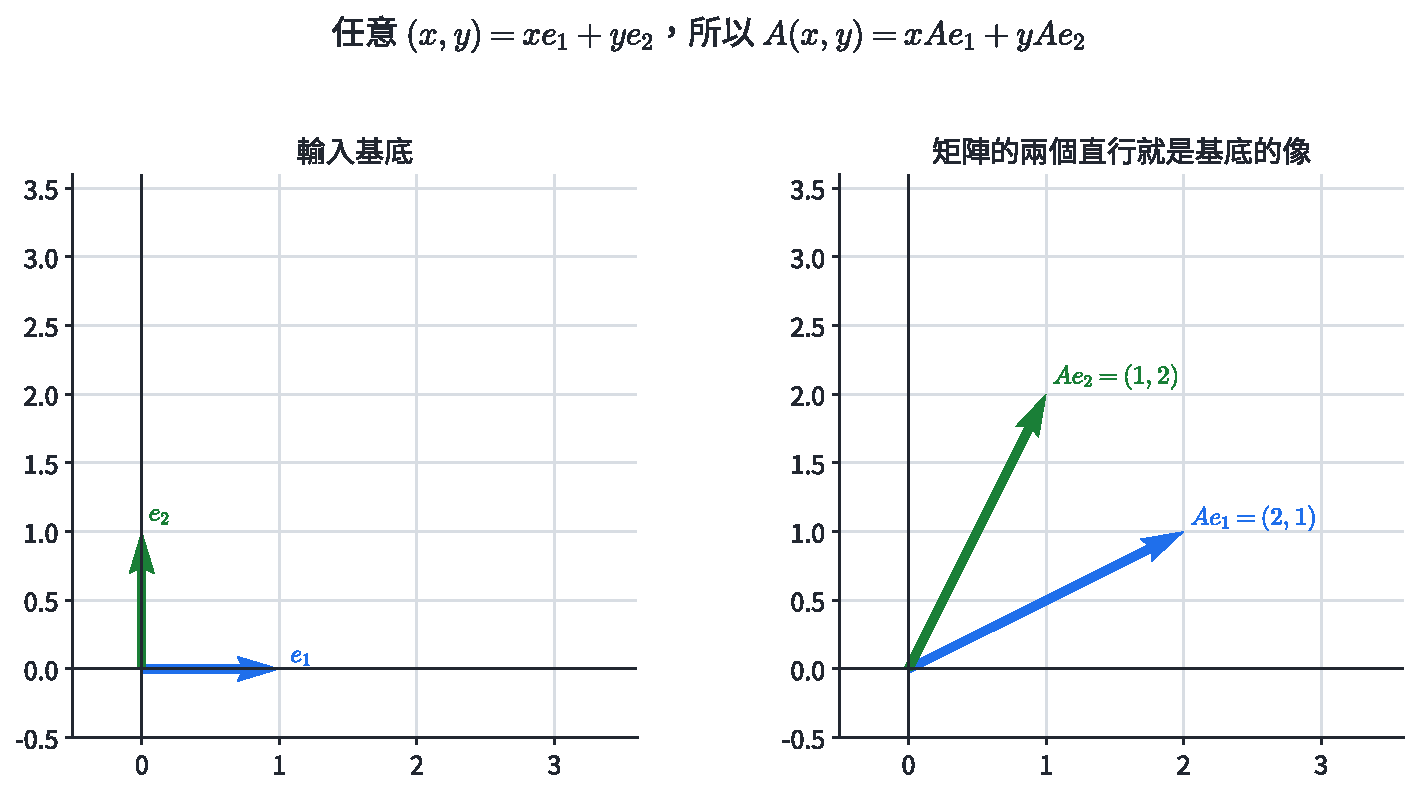
\includegraphics[width=0.94\linewidth,height=\textheight,keepaspectratio,alt={圖 11｜矩陣的兩個直行是標準基底的像；任意向量的像由同一組係數線性組合。}]{assets/數A4-4-基底決定變換.pdf}
\caption{圖 11｜矩陣的兩個直行是標準基底的像；任意向量的像由同一組係數線性組合。}
\end{figure}

\begin{HandoutWorkedExample}

\subsection{完整示範｜由基底的像建立矩陣}\label{ux5b8cux6574ux793aux7bc4ux7531ux57faux5e95ux7684ux50cfux5efaux7acbux77e9ux9663}

已知線性變換滿足

\[
T(e_1)=\begin{bmatrix}2\\-1\end{bmatrix},
\qquad
T(e_2)=\begin{bmatrix}3\\4\end{bmatrix}.
\]

因此

\[
A=\boxed{\begin{bmatrix}2&3\\-1&4\end{bmatrix}}.
\]

若 \(v=(5,-2)^T=5e_1-2e_2\)，則

\[
T(v)=5T(e_1)-2T(e_2)
=
\begin{bmatrix}10\\-5\end{bmatrix}
-
\begin{bmatrix}6\\8\end{bmatrix}
=\boxed{\begin{bmatrix}4\\-13\end{bmatrix}}.
\]

直接計算 \(Av\) 得到相同結果。

\end{HandoutWorkedExample}

\begin{HandoutWorkedExample}

\subsection{完整示範｜驗證線性結構}\label{ux5b8cux6574ux793aux7bc4ux9a57ux8b49ux7ddaux6027ux7d50ux69cb}

設

\[
A=\begin{bmatrix}1&2\\3&-1\end{bmatrix},
\quad
u=\begin{bmatrix}2\\1\end{bmatrix},
\quad
v=\begin{bmatrix}-1\\4\end{bmatrix}.
\]

先算

\[
T(u)=\begin{bmatrix}4\\5\end{bmatrix},
\qquad
T(v)=\begin{bmatrix}7\\-7\end{bmatrix}.
\]

另一方面，

\[
T(u+v)
=A\begin{bmatrix}1\\5\end{bmatrix}
=\begin{bmatrix}11\\-2\end{bmatrix}
=T(u)+T(v).
\]

矩陣乘法對向量加法與係數積的分配律，使直線、平行關係與線性組合在變換後仍保持線性結構。

\end{HandoutWorkedExample}

\subsection{6.2 圖形、面積與反像}\label{ux5716ux5f62ux9762ux7a4dux8207ux53cdux50cf}

多邊形經線性變換時，把每個頂點乘上同一矩陣，再依原順序連接。所有面積都乘上 \(|\det A|\)。若 \(\det A\ne0\)，輸出點 \(q\) 的唯一原像為

\[
p=A^{-1}q.
\]

若 \(\det A=0\)，平面被壓縮到一條線或一個點。像集合外的輸出沒有原像；像集合內的每個輸出都有無限多個原像。

\begin{HandoutWorkedExample}

\subsection{完整示範｜變換三角形並核對面積}\label{ux5b8cux6574ux793aux7bc4ux8b8aux63dbux4e09ux89d2ux5f62ux4e26ux6838ux5c0dux9762ux7a4d}

三角形頂點為

\[
O=(0,0),\quad P=(2,0),\quad Q=(0,1),
\]

面積為 \(1\)。令

\[
A=\begin{bmatrix}2&1\\1&3\end{bmatrix}.
\]

各頂點的像為

\[
O'=(0,0),\quad P'=(4,2),\quad Q'=(1,3).
\]

\(|\det A|=|6-1|=5\)，所以新三角形面積為 \(\boxed{5}\)。也可由兩邊向量 \((4,2)\)、\((1,3)\) 的行列式直接驗算：

\[
\frac12|4(3)-2(1)|=5.
\]

\end{HandoutWorkedExample}

\begin{HandoutWorkedExample}

\subsection{完整示範｜由觀測位置求原位置}\label{ux5b8cux6574ux793aux7bc4ux7531ux89c0ux6e2cux4f4dux7f6eux6c42ux539fux4f4dux7f6e}

某坐標校正把原向量 \(p\) 轉成

\[
q=
\begin{bmatrix}3&1\\1&2\end{bmatrix}p.
\]

若觀測到 \(q=(11,8)^T\)，則

\[
\begin{bmatrix}3&1\\1&2\end{bmatrix}^{-1}
=\frac15\begin{bmatrix}2&-1\\-1&3\end{bmatrix},
\]

所以

\[
p=\frac15
\begin{bmatrix}2&-1\\-1&3\end{bmatrix}
\begin{bmatrix}11\\8\end{bmatrix}
=\frac15\begin{bmatrix}14\\13\end{bmatrix}.
\]

因此原位置為

\[
\boxed{p=\left(\frac{14}{5},\frac{13}{5}\right)}.
\]

代回矩陣乘法可得 \((11,8)^T\)。

\end{HandoutWorkedExample}

\begin{HandoutSelfCheck}

\subsection{分節練習｜線性變換}\label{ux5206ux7bc0ux7df4ux7fd2ux7ddaux6027ux8b8aux63db}

\begin{enumerate}
\def\labelenumi{\arabic{enumi}.}
\tightlist
\item
  已知 \(T(e_1)=(1,3)^T\)、\(T(e_2)=(-2,4)^T\)，寫出矩陣並求 \(T(2,-1)\)。
\item
  設 \(A=\begin{bmatrix}2&0\\1&-1\end{bmatrix}\)，求點 \(P(3,2)\) 的像。
\item
  三角形面積為 \(7\)，經 \(A=\begin{bmatrix}1&2\\3&4\end{bmatrix}\) 變換後，求面積。
\item
  求 \(A=\begin{bmatrix}2&1\\1&1\end{bmatrix}\) 將哪個點送到 \((8,5)\)。
\item
  矩形四點為 \((0,0),(2,0),(2,1),(0,1)\)。經 \(A=\begin{bmatrix}1&1\\0&2\end{bmatrix}\) 後，寫出四個像並求面積。
\item
  設 \(B=\begin{bmatrix}1&2\\2&4\end{bmatrix}\)。求 \(B(2,-1)^T\)，並找另一個不同輸入也得到同一輸出。
\end{enumerate}

\textbf{解答}

\begin{enumerate}
\def\labelenumi{\arabic{enumi}.}
\tightlist
\item
  \(A=\begin{bmatrix}1&-2\\3&4\end{bmatrix}\)，\(\boxed{T(2,-1)=(4,2)^T}\)。
\item
  \(\boxed{P'=(6,1)}\)。
\item
  面積倍率 \(|\det A|=2\)，新面積為 \(\boxed{14}\)。
\item
  \(A^{-1}=\begin{bmatrix}1&-1\\-1&2\end{bmatrix}\)，原點為 \(\boxed{(3,2)}\)。
\item
  四個像依序為 \(\boxed{(0,0),(2,0),(3,2),(1,2)}\)；面積倍率為 \(2\)，原面積 \(2\)，新面積 \(\boxed{4}\)。
\item
  \(B(2,-1)^T=(0,0)^T\)；例如 \((0,0)^T\) 也得到同一輸出。這對應 \(\det B=0\) 的壓縮。
\end{enumerate}

\end{HandoutSelfCheck}

\section{7. 伸縮、鏡射、旋轉、推移與合成}\label{ux4f38ux7e2eux93e1ux5c04ux65cbux8f49ux63a8ux79fbux8207ux5408ux6210}

\subsection{7.1 由坐標規則讀出矩陣}\label{ux7531ux5750ux6a19ux898fux5247ux8b80ux51faux77e9ux9663}

常見平面線性變換可直接由 \(x',y'\) 的係數讀成矩陣：

{\def\LTcaptype{none} % do not increment counter
\begin{longtable}[]{@{}
  >{\raggedright\arraybackslash}p{(\linewidth - 4\tabcolsep) * \real{0.3333}}
  >{\raggedright\arraybackslash}p{(\linewidth - 4\tabcolsep) * \real{0.3333}}
  >{\raggedright\arraybackslash}p{(\linewidth - 4\tabcolsep) * \real{0.3333}}@{}}
\toprule\noalign{}
\begin{minipage}[b]{\linewidth}\raggedright
變換
\end{minipage} & \begin{minipage}[b]{\linewidth}\raggedright
坐標規則
\end{minipage} & \begin{minipage}[b]{\linewidth}\raggedright
矩陣
\end{minipage} \\
\midrule\noalign{}
\endhead
\bottomrule\noalign{}
\endlastfoot
沿坐標軸伸縮 & \(x'=hx,\ y'=ky\) & \(\begin{bmatrix}h&0\\0&k\end{bmatrix}\) \\
對 \(x\) 軸鏡射 & \(x'=x,\ y'=-y\) & \(\begin{bmatrix}1&0\\0&-1\end{bmatrix}\) \\
逆時針旋轉 \(\theta\) & \(x'=x\cos\theta-y\sin\theta,\ y'=x\sin\theta+y\cos\theta\) & \(\begin{bmatrix}\cos\theta&-\sin\theta\\\sin\theta&\cos\theta\end{bmatrix}\) \\
沿 \(x\) 方向推移 & \(x'=x+ky,\ y'=y\) & \(\begin{bmatrix}1&k\\0&1\end{bmatrix}\) \\
沿 \(y\) 方向推移 & \(x'=x,\ y'=kx+y\) & \(\begin{bmatrix}1&0\\k&1\end{bmatrix}\) \\
\end{longtable}
}

本章的「推移」是保持原點不動的剪切。一般平移 \((x,y)\mapsto(x+a,y+b)\) 含常數項，屬於仿射變換；延伸課程可用 \(3\times3\) 齊次坐標統一表示。

旋轉矩陣的兩個直行分別是

\[
R_\theta e_1=(\cos\theta,\sin\theta)^T,
\qquad
R_\theta e_2=(-\sin\theta,\cos\theta)^T,
\]

也就是兩個互相垂直、長度為 \(1\) 的旋轉後基底，因此旋轉保持長度與面積。

\begin{figure}
\centering
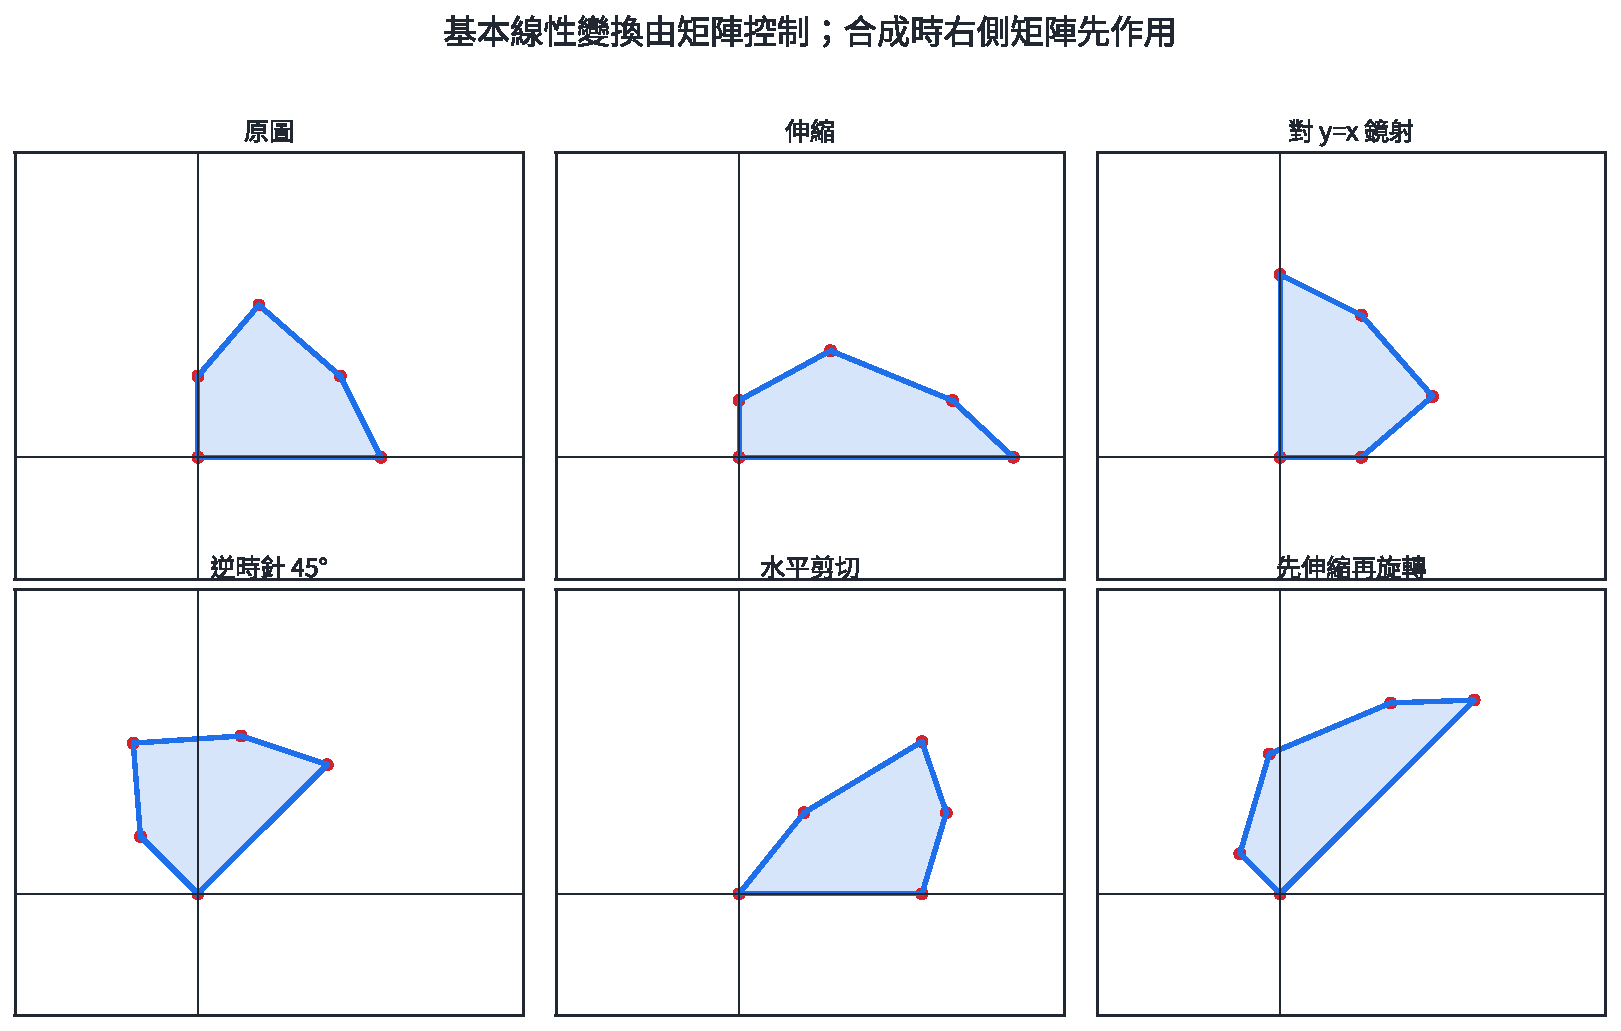
\includegraphics[width=0.97\linewidth,height=\textheight,keepaspectratio,alt={圖 12｜伸縮、鏡射、旋轉與剪切各自改變基底及單位正方形；合成時由右側變換先作用。}]{assets/數A4-4-特殊變換與合成.pdf}
\caption{圖 12｜伸縮、鏡射、旋轉與剪切各自改變基底及單位正方形；合成時由右側變換先作用。}
\end{figure}

\begin{HandoutWorkedExample}

\subsection{完整示範｜旋轉矩陣由基底方向決定}\label{ux5b8cux6574ux793aux7bc4ux65cbux8f49ux77e9ux9663ux7531ux57faux5e95ux65b9ux5411ux6c7aux5b9a}

逆時針旋轉 \(90^\circ\) 時，

\[
e_1\mapsto e_2=(0,1)^T,
\qquad
e_2\mapsto -e_1=(-1,0)^T.
\]

所以

\[
R_{90^\circ}
=\begin{bmatrix}0&-1\\1&0\end{bmatrix}.
\]

點 \(P(3,-2)\) 的像為

\[
R_{90^\circ}\begin{bmatrix}3\\-2\end{bmatrix}
=\boxed{\begin{bmatrix}2\\3\end{bmatrix}}.
\]

原長度與新長度都為 \(\sqrt{13}\)。

\end{HandoutWorkedExample}

\begin{HandoutWorkedExample}

\subsection{完整示範｜對過原點直線的鏡射}\label{ux5b8cux6574ux793aux7bc4ux5c0dux904eux539fux9edeux76f4ux7ddaux7684ux93e1ux5c04}

對與 \(x\) 軸夾角為 \(\theta\) 的直線鏡射，可先旋轉 \(-\theta\) 把鏡線送到 \(x\) 軸，做 \(x\) 軸鏡射，再旋轉 \(\theta\) 回去。化簡後矩陣為

\[
H_\theta=
\begin{bmatrix}
\cos2\theta&\sin2\theta\\
\sin2\theta&-\cos2\theta
\end{bmatrix}.
\]

對直線 \(y=x\) 鏡射時 \(\theta=45^\circ\)，故

\[
H_{45^\circ}
=\begin{bmatrix}0&1\\1&0\end{bmatrix}.
\]

它把 \((4,-1)\) 送到 \(\boxed{(-1,4)}\)，正好交換兩坐標。

\end{HandoutWorkedExample}

\subsection{7.2 合成順序與反向復原}\label{ux5408ux6210ux9806ux5e8fux8207ux53cdux5411ux5fa9ux539f}

若先做 \(B\)、再做 \(A\)，令第一次輸出為 \(v_1\)、第二次輸出為 \(v_2\)，則

\[
v_1=Bv,\qquad v_2=Av_1=A(Bv)=(AB)v.
\]

因此合成矩陣是 \(AB\)，右側矩陣先作用。面積倍率相乘：

\[
|\det(AB)|=|\det A|\,|\det B|.
\]

若兩個變換都可逆，復原時順序相反：

\[
(AB)^{-1}=B^{-1}A^{-1}.
\]

\clearpage

\begin{HandoutWorkedExample}

\subsection{完整示範｜先伸縮再旋轉}\label{ux5b8cux6574ux793aux7bc4ux5148ux4f38ux7e2eux518dux65cbux8f49}

先沿 \(x\) 方向放大 \(2\) 倍，再逆時針旋轉 \(90^\circ\)：

\[
S=\begin{bmatrix}2&0\\0&1\end{bmatrix},
\qquad
R=\begin{bmatrix}0&-1\\1&0\end{bmatrix}.
\]

合成矩陣為

\[
RS=
\begin{bmatrix}0&-1\\2&0\end{bmatrix}.
\]

對 \(v=(1,1)^T\)，

\[
RSv=\boxed{(-1,2)^T}.
\]

若交換順序，\(SRv=(-2,1)^T\)，代表另一個幾何操作。合成面積倍率為 \(|\det(RS)|=2\)。

\end{HandoutWorkedExample}

\begin{HandoutWorkedExample}

\subsection{完整示範｜推移後的坐標與面積}\label{ux5b8cux6574ux793aux7bc4ux63a8ux79fbux5f8cux7684ux5750ux6a19ux8207ux9762ux7a4d}

沿 \(x\) 方向推移係數 \(k=2\)：

\[
K=\begin{bmatrix}1&2\\0&1\end{bmatrix}.
\]

它把 \((x,y)\) 送到 \((x+2y,y)\)。例如

\[
K\begin{bmatrix}1\\3\end{bmatrix}
=\boxed{\begin{bmatrix}7\\3\end{bmatrix}}.
\]

\(\det K=1\)，所以面積保持。水平線仍為水平線；不同高度的點水平位移量為 \(2y\)，因此直立邊會傾斜。

\end{HandoutWorkedExample}

\begin{HandoutWorkedExample}

\subsection{完整示範｜由輸入、輸出設計合成變換}\label{ux5b8cux6574ux793aux7bc4ux7531ux8f38ux5165ux8f38ux51faux8a2dux8a08ux5408ux6210ux8b8aux63db}

要先對 \(x\) 軸鏡射，再沿 \(y\) 方向放大 \(3\) 倍。兩個矩陣為

\[
H=\begin{bmatrix}1&0\\0&-1\end{bmatrix},
\qquad
S=\begin{bmatrix}1&0\\0&3\end{bmatrix}.
\]

合成為

\[
SH=\begin{bmatrix}1&0\\0&-3\end{bmatrix}.
\]

點 \((2,-4)\) 先變為 \((2,4)\)，再變為 \(\boxed{(2,12)}\)。行列式為 \(-3\)：面積放大 \(3\) 倍，負號表示定向翻轉。

\end{HandoutWorkedExample}

\begin{HandoutSelfCheck}

\subsection{分節練習｜特殊變換與合成}\label{ux5206ux7bc0ux7df4ux7fd2ux7279ux6b8aux8b8aux63dbux8207ux5408ux6210}

\begin{enumerate}
\def\labelenumi{\arabic{enumi}.}
\tightlist
\item
  寫出沿 \(x\) 方向縮小為 \(\frac12\)、沿 \(y\) 方向放大為 \(3\) 的矩陣，並求 \((4,-2)\) 的像。
\item
  用矩陣求點 \((-3,5)\) 對 \(y=x\) 鏡射後的坐標。
\item
  寫出逆時針旋轉 \(30^\circ\) 的矩陣，求 \((2,0)\) 的像。
\item
  沿 \(y\) 方向推移係數 \(-2\)。寫出矩陣並求 \((3,1)\) 的像。
\item
  先逆時針旋轉 \(90^\circ\)，再對 \(x\) 軸鏡射。求合成矩陣及 \((1,2)\) 的像。
\item
  先做 \(K=\begin{bmatrix}1&2\\0&1\end{bmatrix}\)，再做 \(S=\begin{bmatrix}3&0\\0&1\end{bmatrix}\)。求合成矩陣、面積倍率與反方陣。
\end{enumerate}

\textbf{解答}

\begin{enumerate}
\def\labelenumi{\arabic{enumi}.}
\tightlist
\item
  \(S=\begin{bmatrix}\tfrac12&0\\0&3\end{bmatrix}\)，像為 \(\boxed{(2,-6)}\)。
\item
  使用 \(\begin{bmatrix}0&1\\1&0\end{bmatrix}\)，像為 \(\boxed{(5,-3)}\)。
\item
  \(R=\begin{bmatrix}\tfrac{\sqrt3}{2}&-\tfrac12\\\tfrac12&\tfrac{\sqrt3}{2}\end{bmatrix}\)，像為 \(\boxed{(\sqrt3,1)}\)。
\item
  \(K=\begin{bmatrix}1&0\\-2&1\end{bmatrix}\)，像為 \(\boxed{(3,-5)}\)。
\item
  合成矩陣為 \(\begin{bmatrix}1&0\\0&-1\end{bmatrix}\begin{bmatrix}0&-1\\1&0\end{bmatrix}=\begin{bmatrix}0&-1\\-1&0\end{bmatrix}\)，像為 \(\boxed{(-2,-1)}\)。
\item
  \(SK=\begin{bmatrix}3&6\\0&1\end{bmatrix}\)，面積倍率為 \(\boxed{3}\)，反方陣為 \(\boxed{\begin{bmatrix}\tfrac13&-2\\0&1\end{bmatrix}}\)。
\end{enumerate}

\end{HandoutSelfCheck}

\section{8. 核心整理}\label{ux6838ux5fc3ux6574ux7406}

{\def\LTcaptype{none} % do not increment counter
\begin{longtable}[]{@{}
  >{\raggedright\arraybackslash}p{(\linewidth - 4\tabcolsep) * \real{0.3333}}
  >{\raggedright\arraybackslash}p{(\linewidth - 4\tabcolsep) * \real{0.3333}}
  >{\raggedright\arraybackslash}p{(\linewidth - 4\tabcolsep) * \real{0.3333}}@{}}
\toprule\noalign{}
\begin{minipage}[b]{\linewidth}\raggedright
問題
\end{minipage} & \begin{minipage}[b]{\linewidth}\raggedright
建模方式
\end{minipage} & \begin{minipage}[b]{\linewidth}\raggedright
關鍵判據
\end{minipage} \\
\midrule\noalign{}
\endhead
\bottomrule\noalign{}
\endlastfoot
多元一次方程組 & 增廣矩陣與列運算 & 樞紐、自由變數、矛盾列 \\
同位置資料合併 & 同階矩陣加減或係數積 & 列數、行數都相同 \\
共享類別加權加總 & 矩陣乘法 & 內側維度相同；列乘行 \\
二階變換能否復原 & 行列式與反方陣 & \(\det A\ne0\) \\
同一流動規則重複多期 & \(X_n=A^nX_0\) & 轉移矩陣元素非負、每個直行和為 \(1\) \\
平面向量的線性變換 & \(T(v)=Av\) & 兩個直行分別是 \(T(e_1),T(e_2)\) \\
連續幾何操作 & 合成矩陣 & 右側變換先作用 \\
\end{longtable}
}

高斯消去法與反方陣都能解聯立方程式。消去法可處理一般階數並直接判斷三種解型；二階反方陣適合可逆方陣，還能描述資料復原與幾何反變換。

行列式同時連接兩個觀點：

\[
\det A=0
\quad\Longleftrightarrow\quad
\text{兩個基底像線性相依}
\quad\Longleftrightarrow\quad
\text{面積塌縮}
\quad\Longleftrightarrow\quad
A\text{ 不可逆}.
\]

矩陣乘法則把全章串在一起：資料表中的共享索引被加總，轉移規則以矩陣冪重複，幾何變換依右至左的順序合成。

\section{9. 章末分層題}\label{ux7ae0ux672bux5206ux5c64ux984c}

\subsection{基礎題}\label{ux57faux790eux984c}

\begin{enumerate}
\def\labelenumi{\arabic{enumi}.}
\item
  用高斯消去法解
  \[
  \begin{cases}
  x+y+z=4,\\
  2x-y+z=1,\\
  x+2y-z=4.
  \end{cases}
  \]
\item
  依參數 \(a\) 判斷下列方程組的解型，並在有解時寫出解：
  \[
  \begin{cases}
  x+y+z=2,\\
  2x+ay+2z=4,\\
  x+2y+z=3.
  \end{cases}
  \]
\item
  設 \(A=[a_{ij}]_{2\times3}\)、\(a_{ij}=2i-j\)，且
  \[
  B=\begin{bmatrix}0&1&2\\-1&0&1\end{bmatrix}.
  \]
  求 \(2A+B\)。
\item
  設
  \[
  A=\begin{bmatrix}1&2&-1\\0&3&2\end{bmatrix},
  \qquad
  B=\begin{bmatrix}2&1\\1&0\\4&-2\end{bmatrix}.
  \]
  求 \(AB\)，並寫出乘積階數。
\end{enumerate}

\subsection{熟練題}\label{ux719fux7df4ux984c}

\begin{enumerate}
\def\labelenumi{\arabic{enumi}.}
\setcounter{enumi}{4}
\item
  求
  \[
  A=\begin{bmatrix}4&1\\2&1\end{bmatrix}
  \]
  的行列式與反方陣，並以 \(AA^{-1}=I\) 驗算。
\item
  解矩陣方程式
  \[
  X\begin{bmatrix}1&1\\0&2\end{bmatrix}
  =
  \begin{bmatrix}3&5\\2&6\end{bmatrix}.
  \]
\item
  甲、乙兩個生產批次使用原料一、二的數量矩陣為
  \[
  Q=\begin{bmatrix}5&2\\3&4\end{bmatrix},
  \]
  兩種原料在一月、二月的單價矩陣為
  \[
  P=\begin{bmatrix}20&22\\30&28\end{bmatrix}.
  \]
  求兩批次在兩個月份的原料總成本矩陣，並解釋右下角元素。
\item
  二次函數 \(p(x)=ax^2+bx+c\) 通過 \((0,1),(1,4),(2,11)\)。用聯立方程式求 \(p(x)\)，並求 \(p(3)\)。
\end{enumerate}

\subsection{應用題}\label{ux61c9ux7528ux984c}

\begin{enumerate}
\def\labelenumi{\arabic{enumi}.}
\setcounter{enumi}{8}
\item
  兩狀態轉移矩陣與初始比例為
  \[
  A=\begin{bmatrix}0.7&0.2\\0.3&0.8\end{bmatrix},
  \qquad
  X_0=\begin{bmatrix}0.6\\0.4\end{bmatrix}.
  \]
  求 \(X_1,X_2\)。
\item
  求第 9 題轉移矩陣的穩定比例，並比較 \(X_2\) 與穩定比例各分量的差。
\item
  線性變換滿足
  \[
  T(e_1)=\begin{bmatrix}2\\1\end{bmatrix},
  \qquad
  T(e_2)=\begin{bmatrix}-1\\3\end{bmatrix}.
  \]
  求變換矩陣、\(T(4,-2)\) 與面積倍率。
\item
  先沿 \(x\) 方向推移 \(x'=x+y\)，再逆時針旋轉 \(90^\circ\)。求合成矩陣，並求 \((2,1)\) 的像與面積倍率。
\end{enumerate}

\subsection{跨節整合題}\label{ux8de8ux7bc0ux6574ux5408ux984c}

\begin{enumerate}
\def\labelenumi{\arabic{enumi}.}
\setcounter{enumi}{12}
\item
  某雙通道感測器用兩個純訊號校正。輸入 \((1,0)^T\) 時輸出 \((2,1)^T\)；輸入 \((0,1)^T\) 時輸出 \((1,2)^T\)。

  \begin{enumerate}
  \def\labelenumii{(\arabic{enumii})}
  \tightlist
  \item
    寫出感測矩陣 \(A\)。\\
  \item
    實測輸出為 \((8,7)^T\)，求原始訊號。\\
  \item
    若兩種原始訊號每單位成本分別為 \(40,25\) 元，求這次訊號代表的總成本。
  \end{enumerate}
\item
  兩狀態模型為
  \[
  A(q)=\begin{bmatrix}0.8&q\\0.2&1-q\end{bmatrix}.
  \]
  已知 \(X_0=(0.5,0.5)^T\)、\(X_1=(0.55,0.45)^T\)。

  \begin{enumerate}
  \def\labelenumii{(\arabic{enumii})}
  \tightlist
  \item
    由觀測求 \(q\)。\\
  \item
    求 \(X_2\)。\\
  \item
    求此模型的穩定比例。
  \end{enumerate}
\item
  三角形頂點為 \(O(0,0),P(2,0),Q(0,1)\)。先沿 \(x\) 方向做 \(x'=x+2y\) 的推移，再沿 \(x,y\) 方向分別放大 \(3\) 倍、縮小為 \(\frac12\)。

  \begin{enumerate}
  \def\labelenumii{(\arabic{enumii})}
  \tightlist
  \item
    求合成矩陣。\\
  \item
    求三個頂點的像與新面積。\\
  \item
    若某輸出點為 \((12,1)\)，求其原像。
  \end{enumerate}
\item
  未知線性變換 \(T\) 滿足
  \[
  T(1,1)=(3,4),\qquad T(2,-1)=(3,-1).
  \]

  \begin{enumerate}
  \def\labelenumii{(\arabic{enumii})}
  \tightlist
  \item
    以聯立方程式求 \(T\) 的矩陣。\\
  \item
    求 \(T(3,2)\)。\\
  \item
    求面積倍率，並判斷每個輸出是否有唯一原像。
  \end{enumerate}
\end{enumerate}

\section{10. 章末題完整解析}\label{ux7ae0ux672bux984cux5b8cux6574ux89e3ux6790}

\subsection{第 1 題}\label{ux7b2c-1-ux984c}

增廣矩陣為

\[
\left[
\begin{array}{ccc|c}
1&1&1&4\\
2&-1&1&1\\
1&2&-1&4
\end{array}
\right].
\]

先做

\[
R_2\leftarrow R_2-2R_1,
\]

得到

\[
\left[
\begin{array}{ccc|c}
1&1&1&4\\
0&-3&-1&-7\\
1&2&-1&4
\end{array}
\right].
\]

\clearpage

再做

\[
R_3\leftarrow R_3-R_1,
\]

得到

\[
\left[
\begin{array}{ccc|c}
1&1&1&4\\
0&-3&-1&-7\\
0&1&-2&0
\end{array}
\right].
\]

交換第二、三列：

\[
R_2\leftrightarrow R_3,
\]

\[
\left[
\begin{array}{ccc|c}
1&1&1&4\\
0&1&-2&0\\
0&-3&-1&-7
\end{array}
\right].
\]

最後做

\[
R_3\leftarrow R_3+3R_2,
\]

\[
\left[
\begin{array}{ccc|c}
1&1&1&4\\
0&1&-2&0\\
0&0&-7&-7
\end{array}
\right].
\]

所以 \(z=1\)、\(y=2\)、\(x=1\)，

\[
\boxed{(x,y,z)=(1,2,1)}.
\]

代回三式依序為 \(4,1,4\)。

\subsection{第 2 題}\label{ux7b2c-2-ux984c}

令 \(u=x+z\)。第一、三式成為

\[
u+y=2,\qquad u+2y=3,
\]

相減得 \(y=1\)，再得 \(u=1\)。第二式要求

\[
2u+ay=4
\quad\Longrightarrow\quad
2+a=4.
\]

因此 \(a=2\) 時第二式是第一式的兩倍，且

\[
y=1,\qquad x+z=1.
\]

令 \(z=t\)，解為

\[
\boxed{(x,y,z)=(1-t,1,t),\quad t\in\mathbb R},
\]

共有無限多組。\(a\ne2\) 時，第一、三式已固定 \(u=1,y=1\)，再代入第二式會形成矛盾，故 \(\boxed{\text{無解}}\)。

\subsection{第 3 題}\label{ux7b2c-3-ux984c}

依 \(a_{ij}=2i-j\)，

\[
A=\begin{bmatrix}
1&0&-1\\
3&2&1
\end{bmatrix}.
\]

所以

\[
2A+B
=
\begin{bmatrix}
2&0&-2\\
6&4&2
\end{bmatrix}
+
\begin{bmatrix}
0&1&2\\
-1&0&1
\end{bmatrix}
=
\boxed{\begin{bmatrix}2&1&0\\5&4&3\end{bmatrix}}.
\]

\subsection{第 4 題}\label{ux7b2c-4-ux984c}

\(A\) 為 \(2\times3\)、\(B\) 為 \(3\times2\)，故 \(AB\) 為 \(2\times2\)：

\[
AB=
\begin{bmatrix}
1(2)+2(1)-1(4)&1(1)+2(0)-1(-2)\\
0(2)+3(1)+2(4)&0(1)+3(0)+2(-2)
\end{bmatrix}
=
\boxed{\begin{bmatrix}0&3\\11&-4\end{bmatrix}}.
\]

\subsection{第 5 題}\label{ux7b2c-5-ux984c}

\[
\det A=4(1)-1(2)=2.
\]

因此

\[
\boxed{
A^{-1}
=\frac12\begin{bmatrix}1&-1\\-2&4\end{bmatrix}}.
\]

驗算：

\[
AA^{-1}
=\frac12
\begin{bmatrix}
4-2&-4+4\\
2-2&-2+4
\end{bmatrix}
=I.
\]

\subsection{第 6 題}\label{ux7b2c-6-ux984c}

令

\[
C=\begin{bmatrix}1&1\\0&2\end{bmatrix},
\qquad
C^{-1}=\begin{bmatrix}1&-\tfrac12\\0&\tfrac12\end{bmatrix}.
\]

未知矩陣在乘積左側，因此右乘 \(C^{-1}\)：

\[
X=
\begin{bmatrix}3&5\\2&6\end{bmatrix}
\begin{bmatrix}1&-\tfrac12\\0&\tfrac12\end{bmatrix}
=
\boxed{\begin{bmatrix}3&1\\2&2\end{bmatrix}}.
\]

代回 \(XC\) 得題目的右側矩陣。

\subsection{第 7 題}\label{ux7b2c-7-ux984c}

數量的行索引與單價的列索引同為原料種類，因此

\[
QP=
\begin{bmatrix}5&2\\3&4\end{bmatrix}
\begin{bmatrix}20&22\\30&28\end{bmatrix}
=
\boxed{\begin{bmatrix}160&166\\180&178\end{bmatrix}}.
\]

右下角

\[
3(22)+4(28)=178
\]

表示乙批次按二月單價計算的原料總成本為 \(\boxed{178}\) 元。

\subsection{第 8 題}\label{ux7b2c-8-ux984c}

代入三點：

\[
\begin{cases}
c=1,\\
a+b+c=4,\\
4a+2b+c=11.
\end{cases}
\]

所以

\[
a+b=3,\qquad 2a+b=5.
\]

相減得 \(a=2\)，再得 \(b=1\)。因此

\[
\boxed{p(x)=2x^2+x+1},
\qquad
\boxed{p(3)=22}.
\]

\subsection{第 9 題}\label{ux7b2c-9-ux984c}

\[
X_1=AX_0
=
\begin{bmatrix}
0.7(0.6)+0.2(0.4)\\
0.3(0.6)+0.8(0.4)
\end{bmatrix}
=
\boxed{\begin{bmatrix}0.5\\0.5\end{bmatrix}}.
\]

再作用一次：

\[
X_2=AX_1
=
\begin{bmatrix}
0.7(0.5)+0.2(0.5)\\
0.3(0.5)+0.8(0.5)
\end{bmatrix}
=
\boxed{\begin{bmatrix}0.45\\0.55\end{bmatrix}}.
\]

兩期的分量和都為 \(1\)。

\clearpage

\subsection{第 10 題}\label{ux7b2c-10-ux984c}

令穩定比例為 \((x,y)^T\)。由

\[
0.7x+0.2y=x
\]

得 \(0.3x=0.2y\)，所以 \(x:y=2:3\)。配合 \(x+y=1\)：

\[
\boxed{X_*=\begin{bmatrix}0.4\\0.6\end{bmatrix}}.
\]

與第 9 題算得的 \(X_2=(0.45,0.55)^T\) 比較：

\[
X_2-X_*=
\begin{bmatrix}0.05\\-0.05\end{bmatrix}.
\]

也就是第一狀態仍高 \(0.05\)，第二狀態仍低 \(0.05\)。

\subsection{第 11 題}\label{ux7b2c-11-ux984c}

兩個基底的像依序放入矩陣直行：

\[
A=\boxed{\begin{bmatrix}2&-1\\1&3\end{bmatrix}}.
\]

\[
T(4,-2)
=
A\begin{bmatrix}4\\-2\end{bmatrix}
=
\boxed{\begin{bmatrix}10\\-2\end{bmatrix}}.
\]

面積倍率為

\[
|\det A|=|2(3)-(-1)(1)|=\boxed{7}.
\]

\subsection{第 12 題}\label{ux7b2c-12-ux984c}

推移與旋轉矩陣為

\[
K=\begin{bmatrix}1&1\\0&1\end{bmatrix},
\qquad
R=\begin{bmatrix}0&-1\\1&0\end{bmatrix}.
\]

先 \(K\) 後 \(R\)，所以合成矩陣為

\[
RK=
\boxed{\begin{bmatrix}0&-1\\1&1\end{bmatrix}}.
\]

\[
RK\begin{bmatrix}2\\1\end{bmatrix}
=\boxed{\begin{bmatrix}-1\\3\end{bmatrix}}.
\]

面積倍率為 \(|\det(RK)|=\boxed{1}\)。

\subsection{第 13 題}\label{ux7b2c-13-ux984c}

純訊號就是標準基底，因此兩個校正輸出是矩陣的兩個直行：

\[
\boxed{A=\begin{bmatrix}2&1\\1&2\end{bmatrix}}.
\]

\(\det A=3\)，故

\[
A^{-1}=\frac13\begin{bmatrix}2&-1\\-1&2\end{bmatrix}.
\]

原始訊號為

\[
x=A^{-1}\begin{bmatrix}8\\7\end{bmatrix}
=\frac13
\begin{bmatrix}16-7\\-8+14\end{bmatrix}
=
\boxed{\begin{bmatrix}3\\2\end{bmatrix}}.
\]

成本為

\[
\begin{bmatrix}40&25\end{bmatrix}
\begin{bmatrix}3\\2\end{bmatrix}
=120+50
=\boxed{170\text{ 元}}.
\]

代回 \(A(3,2)^T=(8,7)^T\)，校正與復原一致。

\subsection{第 14 題}\label{ux7b2c-14-ux984c}

第一期第一分量給出

\[
0.8(0.5)+q(0.5)=0.55,
\]

所以

\[
\boxed{q=0.3}.
\]

此時

\[
A=\begin{bmatrix}0.8&0.3\\0.2&0.7\end{bmatrix}.
\]

第二期為

\[
X_2=AX_1
=
\begin{bmatrix}
0.8(0.55)+0.3(0.45)\\
0.2(0.55)+0.7(0.45)
\end{bmatrix}
=
\boxed{\begin{bmatrix}0.575\\0.425\end{bmatrix}}.
\]

穩定比例滿足

\[
0.8x+0.3y=x
\quad\Longrightarrow\quad
0.2x=0.3y.
\]

配合 \(x+y=1\)，得到

\[
\boxed{X_*=(0.6,0.4)^T}.
\]

\subsection{第 15 題}\label{ux7b2c-15-ux984c}

推移與伸縮矩陣為

\[
K=\begin{bmatrix}1&2\\0&1\end{bmatrix},
\qquad
S=\begin{bmatrix}3&0\\0&\tfrac12\end{bmatrix}.
\]

先 \(K\) 後 \(S\)：

\[
A=SK
=
\boxed{\begin{bmatrix}3&6\\0&\tfrac12\end{bmatrix}}.
\]

三個頂點的像為

\[
O'=(0,0),\qquad
P'=A(2,0)^T=(6,0),\qquad
Q'=A(0,1)^T=\left(6,\tfrac12\right).
\]

原三角形面積為 \(1\)，面積倍率為

\[
|\det A|=\left|3\cdot\frac12\right|=\frac32,
\]

故新面積為 \(\boxed{\frac32}\)。

反方陣為

\[
A^{-1}=
\begin{bmatrix}\tfrac13&-4\\0&2\end{bmatrix}.
\]

輸出 \((12,1)^T\) 的原像為

\[
A^{-1}\begin{bmatrix}12\\1\end{bmatrix}
=
\begin{bmatrix}4-4\\2\end{bmatrix}
=\boxed{\begin{bmatrix}0\\2\end{bmatrix}}.
\]

\clearpage

\subsection{第 16 題}\label{ux7b2c-16-ux984c}

設

\[
A=\begin{bmatrix}a&b\\c&d\end{bmatrix}.
\]

由兩組輸入輸出，

\[
\begin{cases}
a+b=3,\\
2a-b=3,
\end{cases}
\qquad
\begin{cases}
c+d=4,\\
2c-d=-1.
\end{cases}
\]

前一組相加得 \(3a=6\)，所以 \(a=2,b=1\)；後一組相加得 \(3c=3\)，所以 \(c=1,d=3\)。因此

\[
\boxed{A=\begin{bmatrix}2&1\\1&3\end{bmatrix}}.
\]

\[
T(3,2)
=A\begin{bmatrix}3\\2\end{bmatrix}
=
\boxed{\begin{bmatrix}8\\9\end{bmatrix}}.
\]

行列式為 \(\det A=2(3)-1(1)=5\)，所以面積倍率為 \(\boxed{5}\)，且 \(\det A\ne0\)，反方陣存在，每個輸出都有唯一原像。


\end{document}
